\documentclass{article}
\usepackage[letterpaper, margin=1in]{geometry}
\usepackage{ragged2e}
\usepackage[hidelinks]{hyperref}
\usepackage{booktabs}
\usepackage{tabularx}
\usepackage{titling}
\usepackage[titletoc,title]{appendix}
\usepackage{setspace}
\usepackage{tikz}
\usepackage{graphicx} % Include graphic importing
\graphicspath{{images/}}
\newcommand{\subtitle}[1]{%
  \posttitle{%
    \par\end{center}
    \begin{center}\large#1\end{center}
    \vskip0.5em}%
}
\usepackage{listings}
\usepackage{color}
\definecolor{dkgreen}{rgb}{0,0.6,0}
\definecolor{gray}{rgb}{0.5,0.5,0.5}
\definecolor{mauve}{rgb}{0.58,0,0.82}
\lstset{frame=tb,
  language=Java,
  aboveskip=3mm,
  belowskip=3mm,
  showstringspaces=false,
  columns=flexible,
  basicstyle={\small\ttfamily},
  numbers=none,
  numberstyle=\tiny\color{gray},
  keywordstyle=\color{blue},
  commentstyle=\color{dkgreen},
  stringstyle=\color{mauve},
  breaklines=true,
  breakatwhitespace=true,
  tabsize=3
}
\usepackage{float}
\usepackage{cite}
\usepackage[final]{pdfpages}

\usepackage[toc,nonumberlist,acronym]{glossaries}
\newglossary[blg]{beer}{bls}{blo}{Beer Terminology}
\newglossary[tlg]{technical}{tls}{tlo}{Technical Terminology}
\makeglossaries

\newglossaryentry{grain-bill}{type=beer,name=Grain Bill, text=grain bill, description=The required amount of grains for the \gls{mash} in order to reach the desired \gls{gravity} necessary for the \gls{wort}.}
\newglossaryentry{gravity}{type=beer,name=Gravity, text=gravity, description=The density of the \gls{wort}.  This is often assumed to be the sugar density of the \gls{wort}.  The term \ensuremath{OG} refers to the original gravity of the \gls{wort}.  \ensuremath{SG} refers to the current specific gravity of the \gls{wort}.  \ensuremath{FG} refers to the final gravity upon the completion of fermentation.  The difference between the \ensuremath{FG} and \ensuremath{OG} is often used to calculate the percentage of alcohol in the final product.}
\newglossaryentry{grist}{type=beer, name=Grist, text=grist, description=The combination of milled grains to be used in a particular brew. Also sometimes applied to hops \cite{beer-terms}.}
\newglossaryentry{lauter}{type=beer, name=Lauter, text=lauter, description=To run the \gls{wort} from the \gls{mash} tun.  From the German word to clarify.  It uses a system of sharp rakes to achieve a very intensive extraction of malt sugars. \cite{beer-terms}.}
\newglossaryentry{mash}{type=beer, name=Mash, text=mash, description=(Verb) To release malt sugars by soaking the grains in water. (Noun) The resultant mixture \cite{beer-terms}.}
\newglossaryentry{pitch}{type=beer, name=Pitch, text=pitch, description=To add yeast.}
\newglossaryentry{sparge}{type=beer, name=Sparge, text=sparge, description=To spray \gls{grist} with hot water in order to remove soluble sugars (maltose). This takes place at the end of the mash \cite{beer-terms}.}
\newglossaryentry{trub}{type=beer, name=Trub, text=trub, description=The layer of sediment that appears at the bottom of the fermentation vessel upon the completion of fermentation.}
\newglossaryentry{wort}{type=beer,name=Wort, text=wort, description=The solution of grain sugars strained from the \gls{mash} tun \cite{beer-terms}.}

\newglossaryentry{rpi}{type=technical, name=Raspberry Pi 2 Model B, text=Raspberry Pi, description=The Raspberry Pi 2 Model B is the second generation Raspberry Pi. It replaced the original Raspberry Pi 1 Model B+ in February 2015.}
\newglossaryentry{ass}{type=technical, name=Austenitic Stainless Steel, description=An alloy family of stainless steels high in \gls{austenite} phase grain structure.}
\newglossaryentry{austenite}{type=technical, name=Austenite, description=A non magnetic crystal structure of iron.  May exist in solid solution with the aid of alloying elements.}
\newglossaryentry{intergrancor}{type=technical, name=Inter-granular Corrosion, description=Corrosion caused by varying composition between the grains and grain boundaries within a metal.  Welding 304 stainless steel may lead to intergranular corrosion if not cooled properly.}
\newglossaryentry{jersey}{type=technical, name=Jersey Framework, description=A \gls{rest} API Framework written in the Java coding language.}
\newglossaryentry{resource}{type=technical, name=Jersey Resource, description=An object with a type\, associated data\, or a set of methods that operate on it.}
\newglossaryentry{ultenstr}{type=technical, name=Ultimate Tensile Strength, description=The maximum tensile stress a material can experience before breaking or fracturing}
\newglossaryentry{yieldstr}{type=technical, name=Yield Stress, description=The stress at which a material begins to plastically deform.}


%\newacronym{abv}{ABV}{Alcohol By Volume}
\newacronym{aisi}{AISI}{American Iron and Steel Institute}
\newacronym{api}{API}{Application Program Interface}
\newacronym{arm}{ARM}{Acorn \gls{risc} Machine}
\newacronym{cfia}{CFIA}{Canadian Food Inspection Agency (CFIA)}
\newacronym{gcm}{GCM}{Google Cloud Messaging}
\newacronym{i2c}{I2C}{Inter-Integrated Circuit}
\newacronym{ide}{IDE}{Integrated Development Environment}
\newacronym{ios}{iOS}{iPhone Operating System}
\newacronym{json}{JSON}{JavaScript Object Notation}
\newacronym{html5}{HTML5}{HyperText Markup Language 5}
\newacronym{lamp}{LAMP}{Lamp Apache MySQL PHP}
\newacronym{lts}{LTS}{Long Term Support}
\newacronym{pid}{PID}{Proportional-Integral-Derivative}
\newacronym{ram}{RAM}{Random Access Memory}
\newacronym{rest}{REST}{RESTful}
\newacronym{risc}{RISC}{Reduced Instruction Set Computing}
\newacronym{ros}{ROS}{Robot Operating System}
\newacronym{sdk}{SDK}{Software Development Kit}
\newacronym{usb}{USB}{Universal Serial Bus}
\newacronym{uri}{URI}{Uniform Resource Identifier}
\newacronym{uts}{UTS}{\gls{ultenstr}}
\newacronym{wlan}{WLAN}{Wireless Local Area Network}
\newacronym{xmpp}{XMPP}{Extensible Messaging and Presence Protocol}

\author{\\\\}
\title{Brew It Yourself}
\subtitle{An Automated Single-Vessel Home Brewery System}

\begin{document}

\begin{titlepage}
    \begin{center}
        \vspace*{1cm}
        
        
        \textsc{\LARGE University of Waterloo}\\ [0.1cm]
        \textsc{\Large Faculty of Engineering}\\
        \textsc{Department of Electrical and Computer Engineering}

		\vspace{4.5cm}

        \textsc{\Huge \textbf{Brew It Yourself}}
        
        \vspace{0.2cm}
        An Automated Single Vessel Home Brewery System
                
        \vfill
        
        Group Number: 2016.019
		\\Consultant: Douglas Harder
        \vspace{0.5cm}
        \\Kevin Nause (20413332) 
        \\Mathieu Tremblay (20420813) 
        \\Scott Wood (20379649) 
        \\Steve Jung (20411563) 
        \vspace{0.5cm}
        \\Date: \today
        \vspace{3.0cm}
    \end{center}
\end{titlepage}

\justify
\onehalfspacing

\pagebreak
\section*{Abstract}

\textbf{Automated Single Vessel Home Brewery System}

The art of home brewing has been steadily gaining popularity over the past 35 years alongside the rise of craft breweries in North America, so much so that in 2010 there were over 2000 craft breweries in the United States, after starting with only 8 in 1980. The objective of this project is
to combine home brewing experience with engineering design, and construct a single vessel brewing system. By maintaining a strict control of key parameters, the brewing process is regulated using a combination of fluid mechanics, heat transfer, digital controls, power systems, embedded robotics and mobile development. The \gls{ros}, allows for a design where sensors can be added to a modular setup and provide feedback. By receiving feedback from temperature readings, density measurements and capacitance monitoring, the brewing process can be accurately recorded, shared, and automated by the system. The single vessel design allows for reduced complexity compared to the traditional home brewing method which requires various components, constant monitoring and heavy maintenance.

\section*{Acknowledgements}
The Brew It Yourself team would like to acknowledge a number of people for providing guidance along the way. Project consultant Douglas Harder, for helping during the brainstorming phase and with interim financial backing; Steve Innocente of Innocente Brewing Company, for providing technical assistance with key problems during the design phase; Andrew Svoboda, for assisting with pre-build trials of the all-grain brewing process; and Rick Forgett and the rest of the Engineering Machine Shop staff, for assisting with the fabrication of our vessel and providing feedback on design decision

\pagebreak

\glsunsetall
\tableofcontents
\pagebreak
\listoffigures
\listoftables
\glsresetall

\pagebreak

\setcounter{section}{0}
\section{High-Level Description of Project}
\subsection{Motivation}
The art of home brewing has been steadily gaining popularity over the past 35 years alongside the rise of craft breweries in North America, so much so that in 2010 there were over 2000 craft breweries in the United States, after starting with only 8 in 1980 \cite{craft-beer}. The traditional method for homebrewing requires various components, constant monitoring and heavy maintenance. There should be a solution which reduces complexity, making it much more affordable and practical for home use. We hope to create a single vessel system that would make the home brewing process precise, automated and compact, all at a reasonable price.
\subsection{Project Objective}
The objective of this project is to combine homebrewing experience with engineering design, and construct a single vessel brewing system. By maintaining a strict control of key parameters, the brewing process is regulated using a combination of fluid mechanics, heat transfer, digital controls, power systems, embedded robotics and mobile development. \gls{ros}, allows for a design where sensors can be added to a modular setup and provide feedback. By receiving feedback from temperature readings, density measurements and pH monitoring, the brewing process can be accurately recorded, shared, and automated by the system. 
\subsection{Block Diagram}
Figure \ref{fig:block} shows relevant links between the physical, mechanical design of the brewing system, as well as the computer systems and their underlying software.

\begin{figure}[H]
\begin{center}
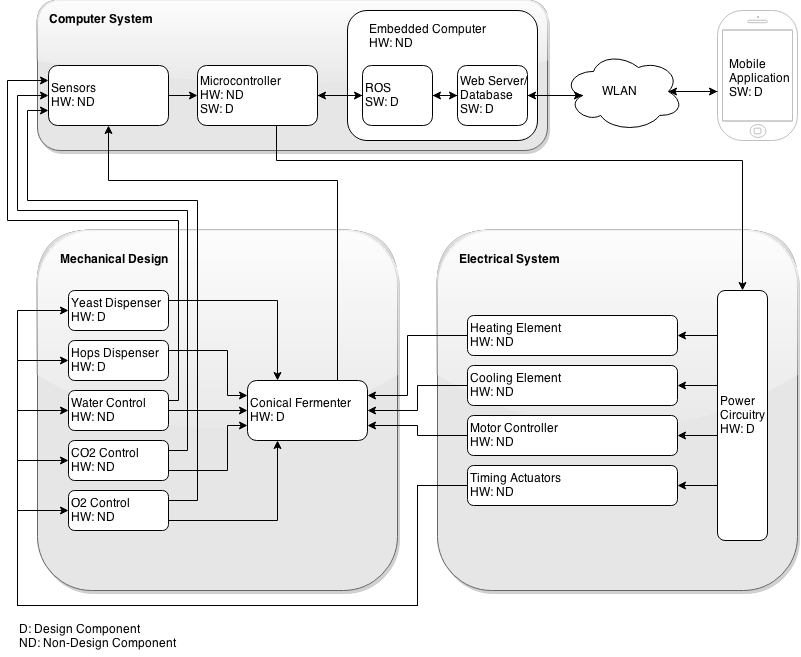
\includegraphics[scale=0.58]{block-diagram.png}
\caption{Block Diagram outlining the interactions between the computer, electrical, and mechanical systems}
\label{fig:block}
\end{center}
\end{figure}

\subsubsection{Description of System}
The single vessel brewing system, as shown in Figure \ref{fig:block}, contains various sensors which forward the environmental parameters to the microcontroller. The data from the various sensors accurately represents the state of the fermenter and feed into digital control loops running on the microcontroller.  Data from sensor modules is obtained by a microcontroller via an \gls{i2c} interface. This data is then sent to an embedded computer system over \gls{usb} where it is logged in a database and used to control relevant subsystems. Control commands are sent from the embedded computer to the microcontroller, where the appropriate component can be communicated with in order to regulate the brewing environment.  The embedded computer system is then able to send diagnostic information and push notifications to a mobile device through a \gls{wlan} connection.

\subsubsection{Designing and Not Designing Components}
The following is an outline of the components in the block diagram and the requirements associated for each Designing (D) and Non-Designing (ND) component.

\begin{itemize}
\item\textbf{Sensors}
\\ND: Sensors being used in the vessel are not being designed.  Instead, off-the-shelf sensors are being purchased and integrated into the system.  Relevant sensor types for this system include, but aren't limited to, pH sensors, volume sensors, flow meters, temperature probes, etc.

\item\textbf{Microcontroller(s)}
\\ND: The hardware of the microcontroller is not being designed since that's outside the scope of this project. The system instead uses an off-the-shelf microcontroller.
D: The software running on the microcontroller is being designed. This software mainly consists of digital control loops for interfacing with the sensors and power electronic circuitry.

\item\textbf{Conical Fermentation Vessel}
\\D: The mechanical features and dimensions of the conical fermentation vessel are being designed to hold various sensors and other electrical and mechanical components. 

\item\textbf{Power Electronic Circuitry}
\\D: The power electronic circuitry is being designed to power the pumps, motors, actuators, and heating/cooling mechanisms. The circuitry takes input from the digital controller running on the microcontroller and outputs the appropriate power to the end devices.

\item\textbf{Heating and Cooling Elements}
\\ND: The heating coils and refrigeration unit used to regulate temperature of the vessel are not being designed. Instead, off-the-shelf or salvaged and adapted components from existing appliances (e.g. hot water tank coils, home air conditioning heat pump) are being used and the power electronic circuitry is being designed to power these devices.

\item\textbf{Motor Controller}
\\ND: The motors, pumps, and mixing mechanisms used in our system are not being designed. Instead, off-the-shelf or salvaged and adapted components from existing appliances (e.g. blender mixing prop, aquarium pumps) are being used and the power electronic circuitry is being designed to power these devices.

\item\textbf{Timing Actuators}
\\ND: The actuators used in our system are not being designed. Instead, off-the-shelf solenoids and servo motors are being used and the mechanical subsystems that they will actuate are being designed. The power electronic circuitry is also being deigned to be able to power the actuators.

\item\textbf{Embedded Computer System}
\\ND: The hardware and operating system of the embedded computer system is not a design objective as it is outside the scope of this project. Instead an off-the-shelf embedded computer is purchased and a Debian based Linux operating system is installed to satisfy the requirements for the development environment.
\\D: The embedded computer system is configured with a Web Server, Database, and \gls{ros}.  Microcontrollers can be modularly added to the system via \gls{usb} and automatically configured as \gls{ros} nodes through negotiations.

\item\textbf{Mobile Application}
\\D: The mobile application is designed such that the user can receive push notifications and see various sensor data during the brew process.
\end{itemize}

\section{Project Specifications}
This section outlines the functional and non-functional requirements of the project design.
\subsection{Functional Specifications}\label{FS}
Table \ref{tab:func} describes each functional requirement and highlights whether it is essential or not to the completion of the project.

\newcolumntype{Z}{>{\raggedright\arraybackslash}X}
\begin{table}[H]
\caption{An overview of each functional specification of the project}
\centering
\begin{tabularx}{\textwidth}{l l Z}
\toprule
\textbf{Specification} & \textbf{Classification} & \textbf{Description} \\ 
\midrule
Completion of the Brewing Process
& Essential	
& The device automatically completes the brewing process, consisting of these steps:
\begin{itemize}
\item \Gls{mash}
\item \Gls{sparge}
\item Boil \Gls{wort}
\item Dispense Hops
\item Aerate the \Gls{wort}
\item \Gls{pitch} the Yeast
\item Kegging and Dispensing
\end{itemize}
\noindent In its entirety and in the correct order.  For more information on the brewing process and the terms used, please see the Glossary.
\\\\
Heating Unit
& Essential
& Mashing the grains, sparging the \gls{grist}, and boiling the \gls{wort} all require high water temperatures. The system is able to accurately heat the contents to a minimum of 110$^{\circ}$C within 3$^{\circ}$C of error.
\\
\end{tabularx}
\end{table}

\begin{table}[H]
\centering
\begin{tabularx}{\textwidth}{l l Z}
Cooling Unit
& Essential
& Yeast pitching and fermentation happen immediately after boiling the \gls{wort}, but require temperatures a specific temperature (typically 20$^{\circ}$C). The system is able to rapidly cool the \gls{wort} to a temperature within 3$^{\circ}$C of the target temperature so that the yeast may be pitched safely.
\\\\
Temperature Regulation
& Essential
& The system is able to control temperature for each step in the brewing process.  An error of 3$^{\circ}$C is the target specification.
\\\\
\Gls{trub} Removal
& Non-Essential
& Remove the undesired sediment and other byproducts at the bottom of the fermenter so that ageing may take place within the vessel.  The user does not have to maintain the \gls{trub} accumulated by the brewing process.
\\\\
Application Notifications
& Non-Essential
& The system provides notifications to the user updating them on the current state or action being taken.  Additionally errors or warnings can be sent, in cases of emergency such as clogs, low oxygen or carbon dioxide, or an improper environment.
\\\\
Database
& Essential
& The system is able query the specific steps it needs to automate for a specific brew.  Additionally, it can store various data involved in brewing including temperature, pH levels and density measurements to generate logs and reports.
\\\\
Reproducibility
& Non-Essential
& The system is able to record recipes, ingredients and steps for various brews. The user can recreate the same type of brew if they select one of the recipes.
\\
\bottomrule
\end{tabularx}
\label{tab:func}
\end{table}

\pagebreak
\subsection{Non-Functional Specifications}
Table \ref{tab:non-func} describes each non-functional requirement and highlights whether it is essential or not to the completion of the project.

\begin{table}[H]
\caption{An overview of each non-functional specification of the project}
\centering
\begin{tabularx}{\textwidth}{l l Z}
\toprule
\textbf{Specification} & \textbf{Classification} & \textbf{Description} \\ 
\midrule
Temperature Accuracy
& Essential
& The system accurately regulates the temperature required for the brewing process within 3$^{\circ}$C of the targeted temperature.
\\\\
Volume Control
& Essential
& The end result must be greater than or equal to the target yield volume.  Target yields typically consist of 15.5 gallons, 7.75 gallons, and 5.16 gallons.  These are the standard sizes of a half barrel keg, quarter barrel keg, and a sixth barrel keg respectively.
\\\\
Size
& Essential
& The dimensions are limited such that the vessel can fit within a standard 36 inch residential door frame.
\\\\
Mobility
& Essential
& The system is able to be relocated by a single person using the aid of caster wheels and or a standard 18 inch wide utility dolly.
\\\\
Sanitation
& Essential
& The system employs SUS 304 stainless steel to maintain food-grade sanitation conditions.  The vessel is self cleaning since a sanitary environment is crucial for the brewing process.
\\
\bottomrule
\end{tabularx}
\label{tab:non-func}
\end{table}
\pagebreak

\section{Detailed Design}
\subsection{Mechanical Design}
The mechanical design component of this project is comprised of two aspects: the structural design of the fermenter and the thermodynamics of the heating and cooling systems.  There are many sources for pre-fabricated fermenters for home brewing, but the custom nature of this device required the construction of a purpose-built tank, shown in Figure \ref{fig:fermenter-wall-cad}.  The tank features a double walled construction to enclose the heating and cooling systems of the inner tank as well as provide thermal insulation.

\begin{figure}[H]
\begin{center}
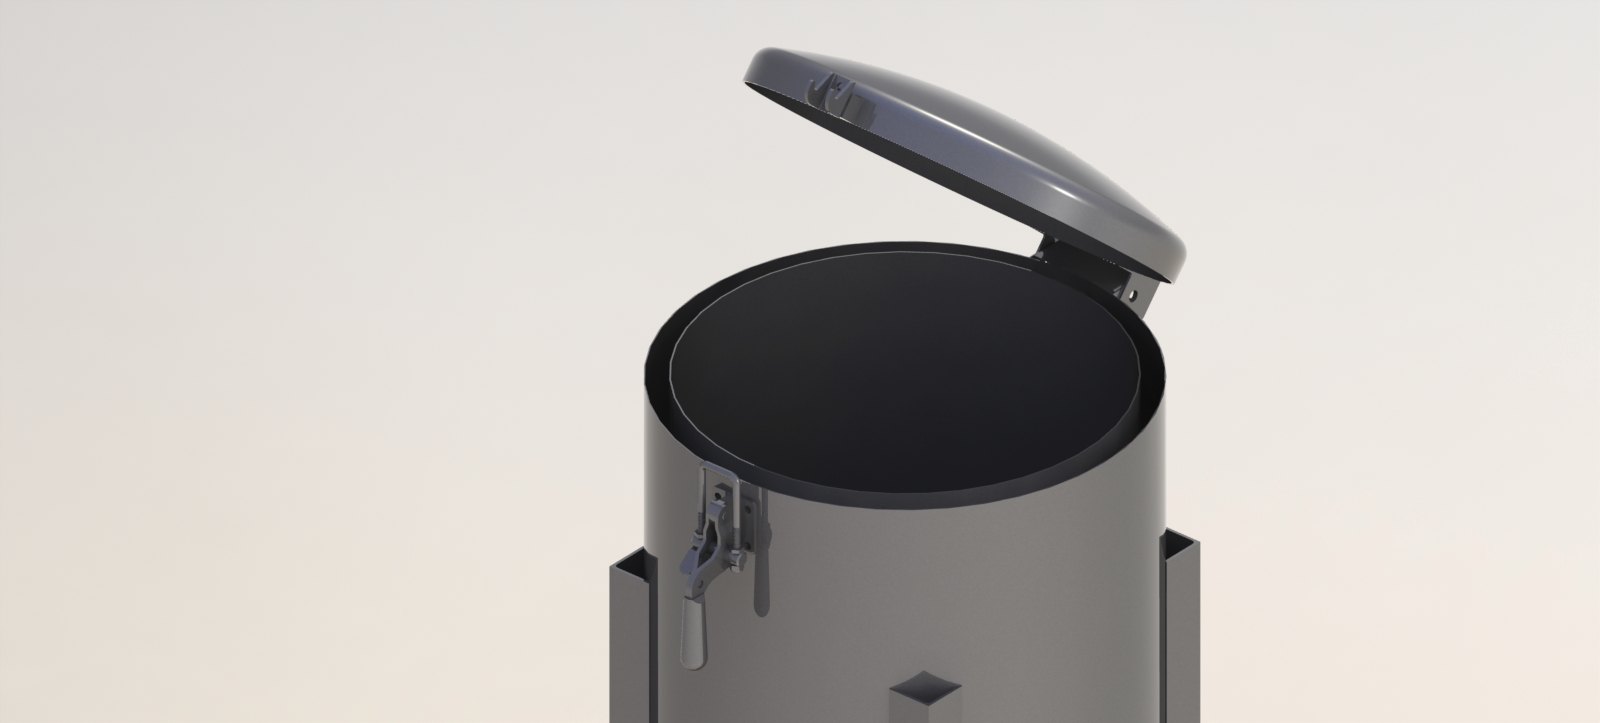
\includegraphics[scale=0.25]{fermenter-wall-cad.png}
\caption{Illustration of the double wall design for the fermenter}
\label{fig:fermenter-wall-cad}
\end{center}
\end{figure}

\subsubsection{Material}
To meet the requirements of food grade equipment, the components of the fermenter that will come into contact with the brewing ingredients are to be constructed from stainless steel.  While the \gls{cfia} does not outline specific details for the materials to be used in food processing, it states that, ``Food contact surfaces of equipment and utensils are smooth, non-corrosive, non-absorbent, non-toxic, free from pitting, cracks or crevices, and able to withstand repeated cleaning and sanitation" \cite{food-grade}.
To meet the non-corrosive guideline set by the \gls{cfia}, \gls{aisi} 304 stainless steel was the specific alloy of stainless steel chosen for the construction of the food-contacting surfaces of the fermenter.  304 is a member of the \gls{ass} family (see \gls{austenite}), which have the best general corrosion resistance of any family of stainless steel.  They also contain low levels of carbon, aiding in weld-ability.  The low levels of carbon also act to reduce the generation of \gls{intergrancor} caused by welding, over the life of the component \cite{asme-eng}.  Tables of the composition of 304 and pertinent mechanical properties are included in \ref{app:304}. The outer tank of the fermenter will not come into contact with the brewing ingredients, and as such, other materials separate from stainless steel may be used.  Aluminium was chosen to be the material for the outer tank due to its low mass and financial cost.

\subsubsection{Tank Structure}
When contemplating the mechanical design for a double-walled system such as this fermenter, the wall thickness for the inner tank should be determined early as this will dictate the structural support required between the inner and outer tanks, as well as the frame to support the entire vessel. Forced carbonation of different brews can reach up to 30psi.  The American Society of Mechanical Engineers (ASME) outlines a function for determining the wall thickness of a pressure vessel as

\begin{equation}
t = \frac{P_{work} \times r \times FS}{\sigma_{uts} \times E}
\end{equation}
\noindent Where: \\
$P$ is the working pressure of the vessel\\
$r$ is the radius of the vessel\\
$FS$ is the factor of safety\\
$­\sigma_{uts}$ is the \gls{uts} of the material\\
$E$ is the non-dimensional efficiency of a welded seam\\

\noindent Therefore:
\begin{equation}
t = \frac{206.84kpa \times 254mm \times 9}{505MPa \times 0.6}
\end{equation}
\begin{equation}
t = 1.560mm
\end{equation}

The recommended thickness derived from this equation is approximately 1/16 of an inch, or 16 gauge when used to describe sheets of stainless steel.
The outer tank thickness can now be specified using the mass of the inner tank and the brewing ingredients.  The design of the system features collars at the top and bottom of both tanks to distribute the load evenly around the perimeter of the outer tank.  The deflection and shear formulas used to determine the forces acting on the tank collars were first introduced in ME 220, Mechanics of Deformable Solids, and ME 322 Machine Design.

\begin{figure}[H]
\begin{center}
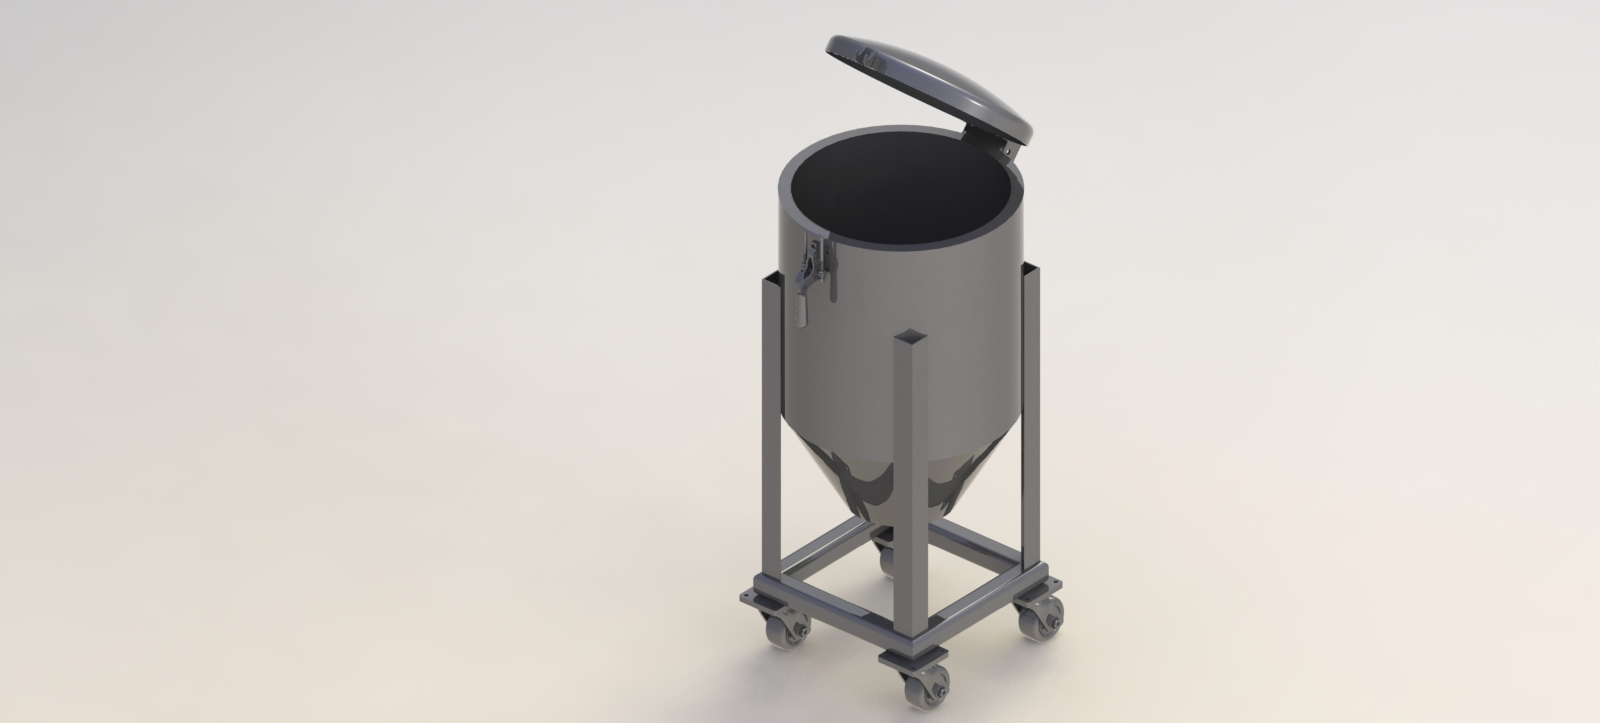
\includegraphics[scale=0.25]{fermenter-cad.png}
\caption{Illustration of the double wall design for the fermenter}
\label{fig:fermenter-cad}
\end{center}
\end{figure}

Formula \ref{eq:stress} was found using the Mechanical Engineer's Handbook \cite{mech-handbook}.
The maximum stress experienced by the collar of the outer tank occurs at the inner edge of the collar.  The \gls{uts} of aluminium can be used as this stress to determine the minimum sheet thickness required to support the fermenter.

\begin{equation}
\sigma = \frac{3w}{mt^{2}(a^{2} - b^{2})}\Big(a^{4}(3m + 1) + b^{4}(m - 1) - 4ma^{2}b^{2} - 4(m + 1)a^{2}b^{2}\ln(\frac{a}{b}) \Big)
\label{eq:stress}
\end{equation}

\noindent Where: \\
$t$ is the sheet thickness\\
$m$ is the reciprocal of Poisson's Ratio\\
$a$ is the outer diameter of the collar\\
$b$ is the inner diameter of the collar\\
$w$ is the applied force on the collar\\

\noindent Therefore:
\begin{equation}
t^{2} = \frac{3w}{m\sigma(a^{2} - b^{2})}\Big(a^{4}(3m + 1) + b^{4}(m - 1) - 4ma^{2}b^{2} - 4(m + 1)a^{2}b^{2}\ln(\frac{a}{b}) \Big)
\end{equation}
The resultant thickness is 2.05mm, or 0.08in. Accounting for a safety factor, a sheet thickness of 0.125in. was selected to meet the requirements for the outer tank.

\subsubsection{Integration of Waste Removal System}
The main challenge following the the design and construction of the structure of the fermenter is the separation of desired brewing products from spent ingredients.  The full rendering below, Figure \ref{fig:full-vessel-render} shows the full fluid circuit.

\begin{figure}[H]
\begin{center}
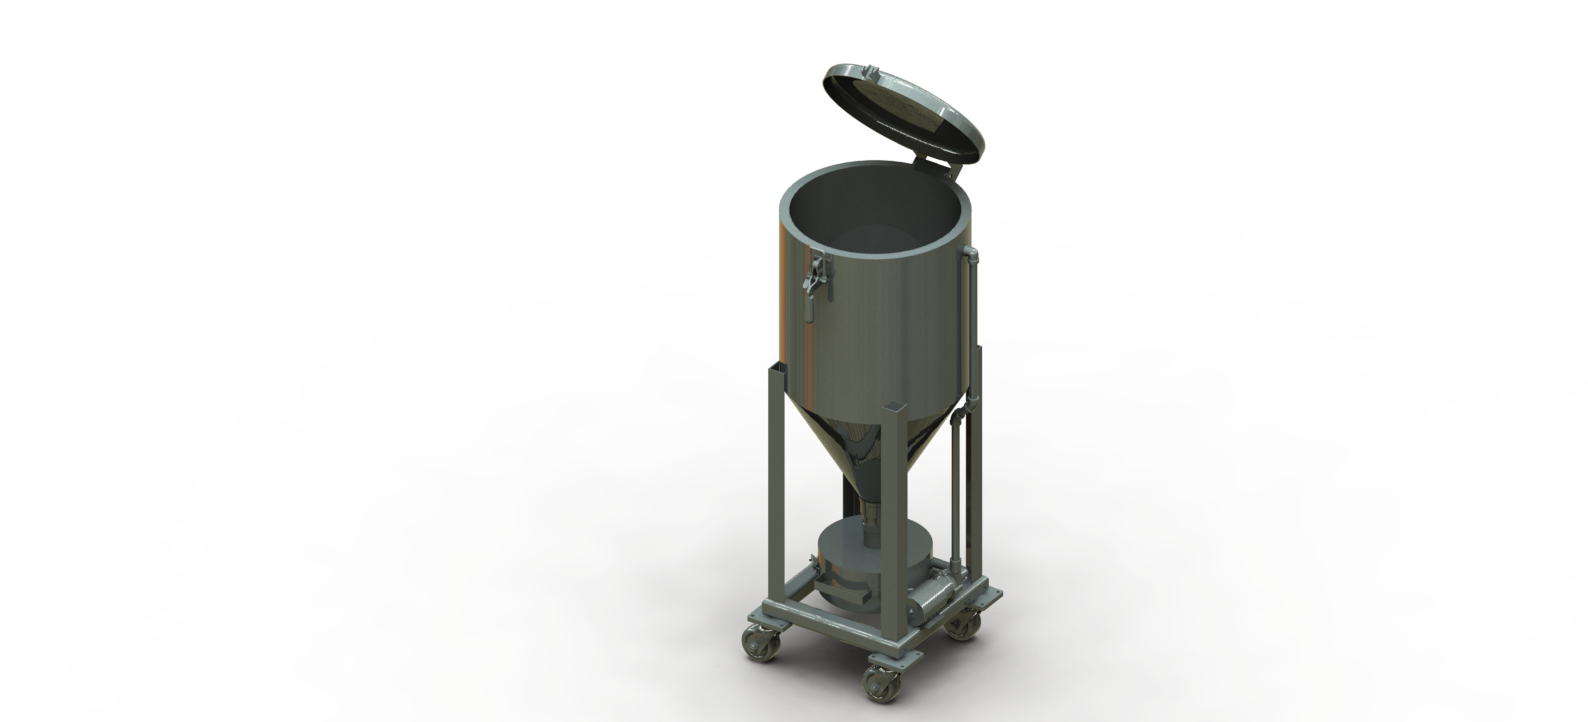
\includegraphics[scale=1]{full-vessel-render.png}
\caption{A render of the full vessel}
\label{fig:full-vessel-render}
\end{center}
\end{figure}

The first step in the process is the removal of the batch from the fermenting vessel. A large, two inch ball valve was selected to mitigate any potential blockage in the system which could be caused by the viscous and tacky \gls{mash}.  After the batch ingredients pass through the valve, they enter into a chamber featuring a wire mesh basket held within the lower container, shown in Figure \ref{fig:filter-basket-render}.

\begin{figure}[H]
\begin{center}
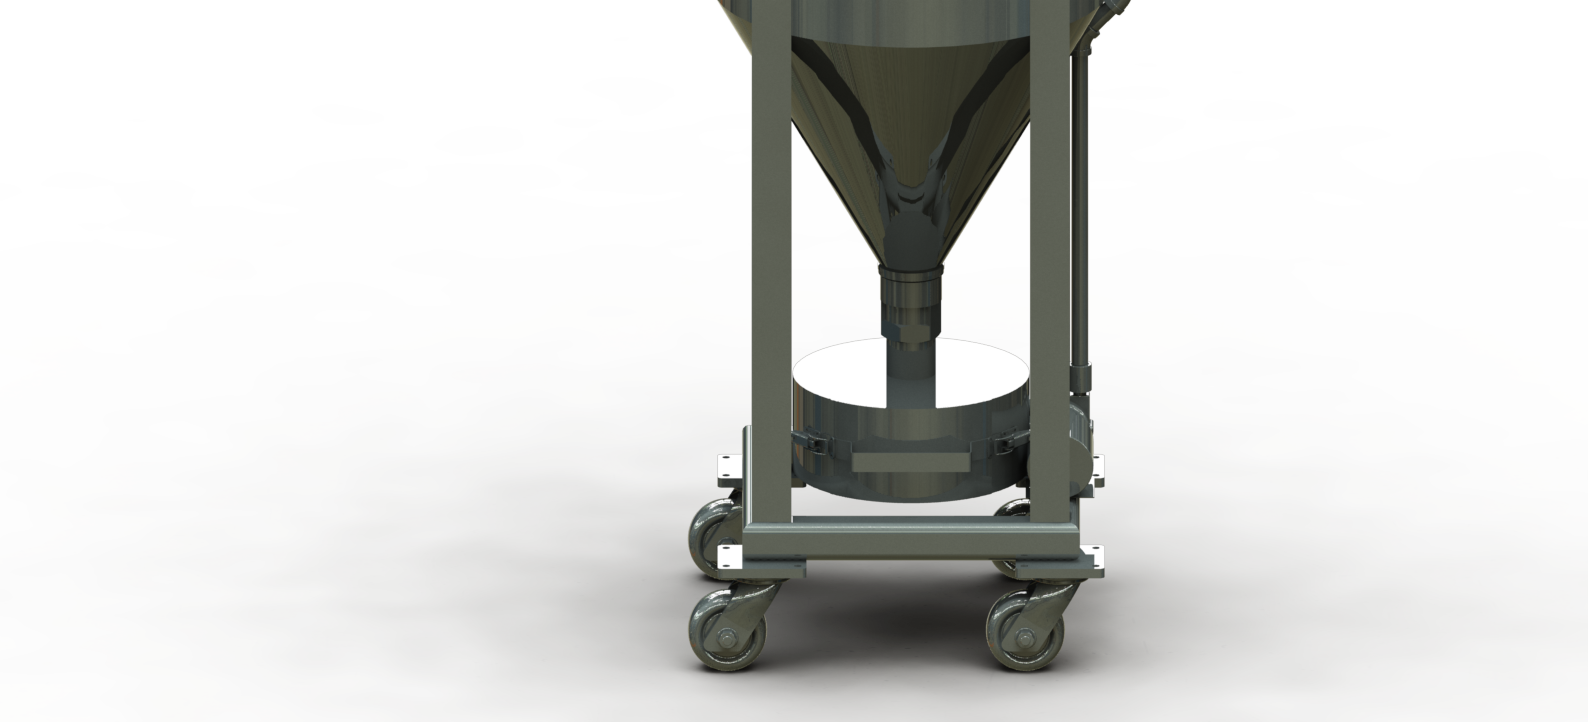
\includegraphics[scale=1]{filter-basket-render.png}
\caption{A render of the filter basket}
\label{fig:filter-basket-render}
\end{center}
\end{figure}

The secondary vessel features a removable, clamp-on door attached to the mesh basket.  This aids with cleanup and preparation for the subsequent brew.  Leftover ingredients and \gls{trub} can be contained in this vessel during the brewing process until the user is ready to remove any waste. A ``Chugger Pump'' is then used to replace the remaining brew into the primary vessel to proceed with fermentation process.  A rendering of the fitment of the pump is shown below in Figure \ref{fig:chugger-pump}.

\begin{figure}[H]
\begin{center}
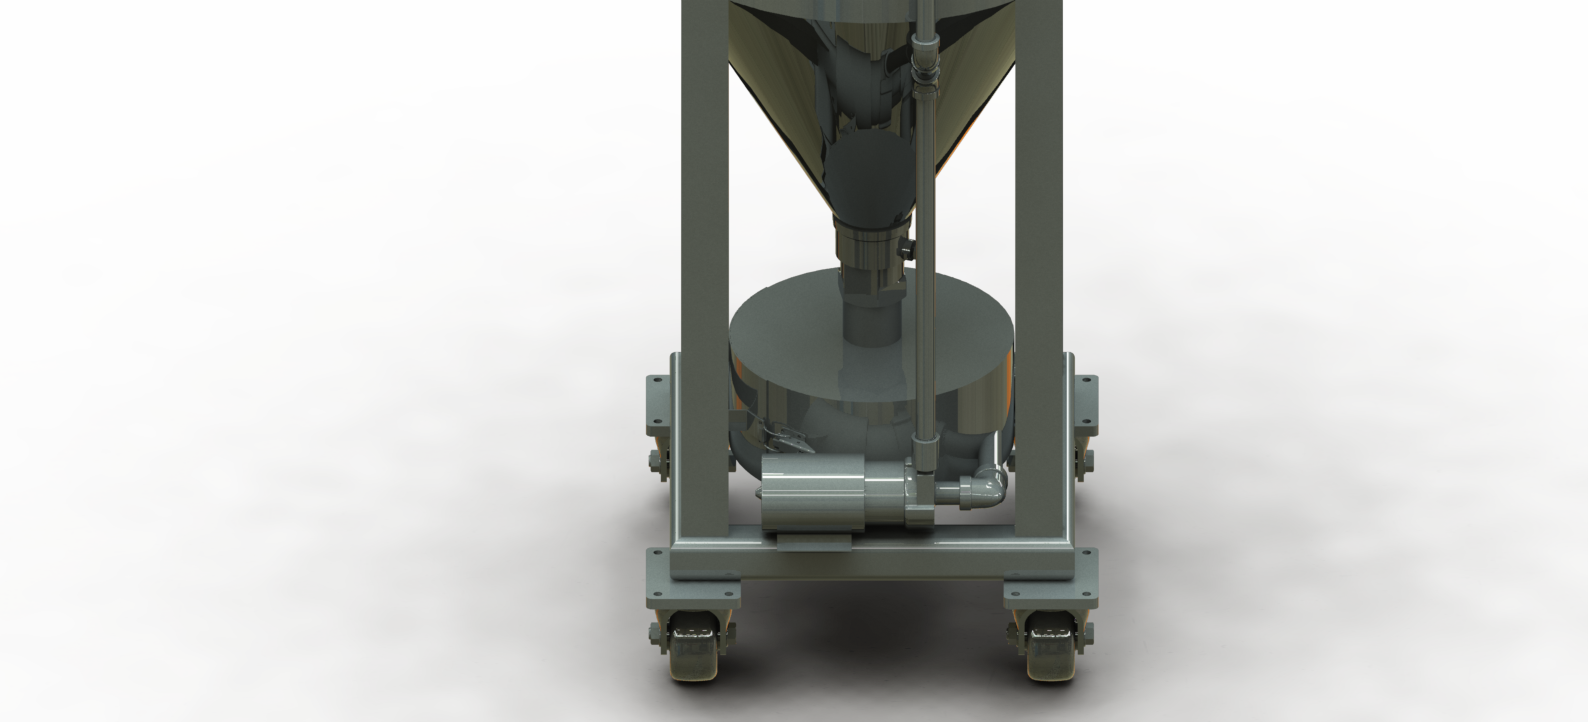
\includegraphics[scale=1]{chugger-pump.png}
\caption{A render of the chugger pump mounting position}
\label{fig:chugger-pump}
\end{center}
\end{figure}

The chugger pump \cite{chugger} was chosen for its durability and resilience, specifically when moving large quantities of sugar rich \gls{wort}.  The integration of these components allows for the completion of an all-grain brew, an increasingly popular method used by contemporary home brewers.

In summary, the mechanical design and renderings contributed to the final mechanical prototype as shown in Figure \ref{fig:mechanical-prototype}.

\begin{figure}[H]
\begin{center}
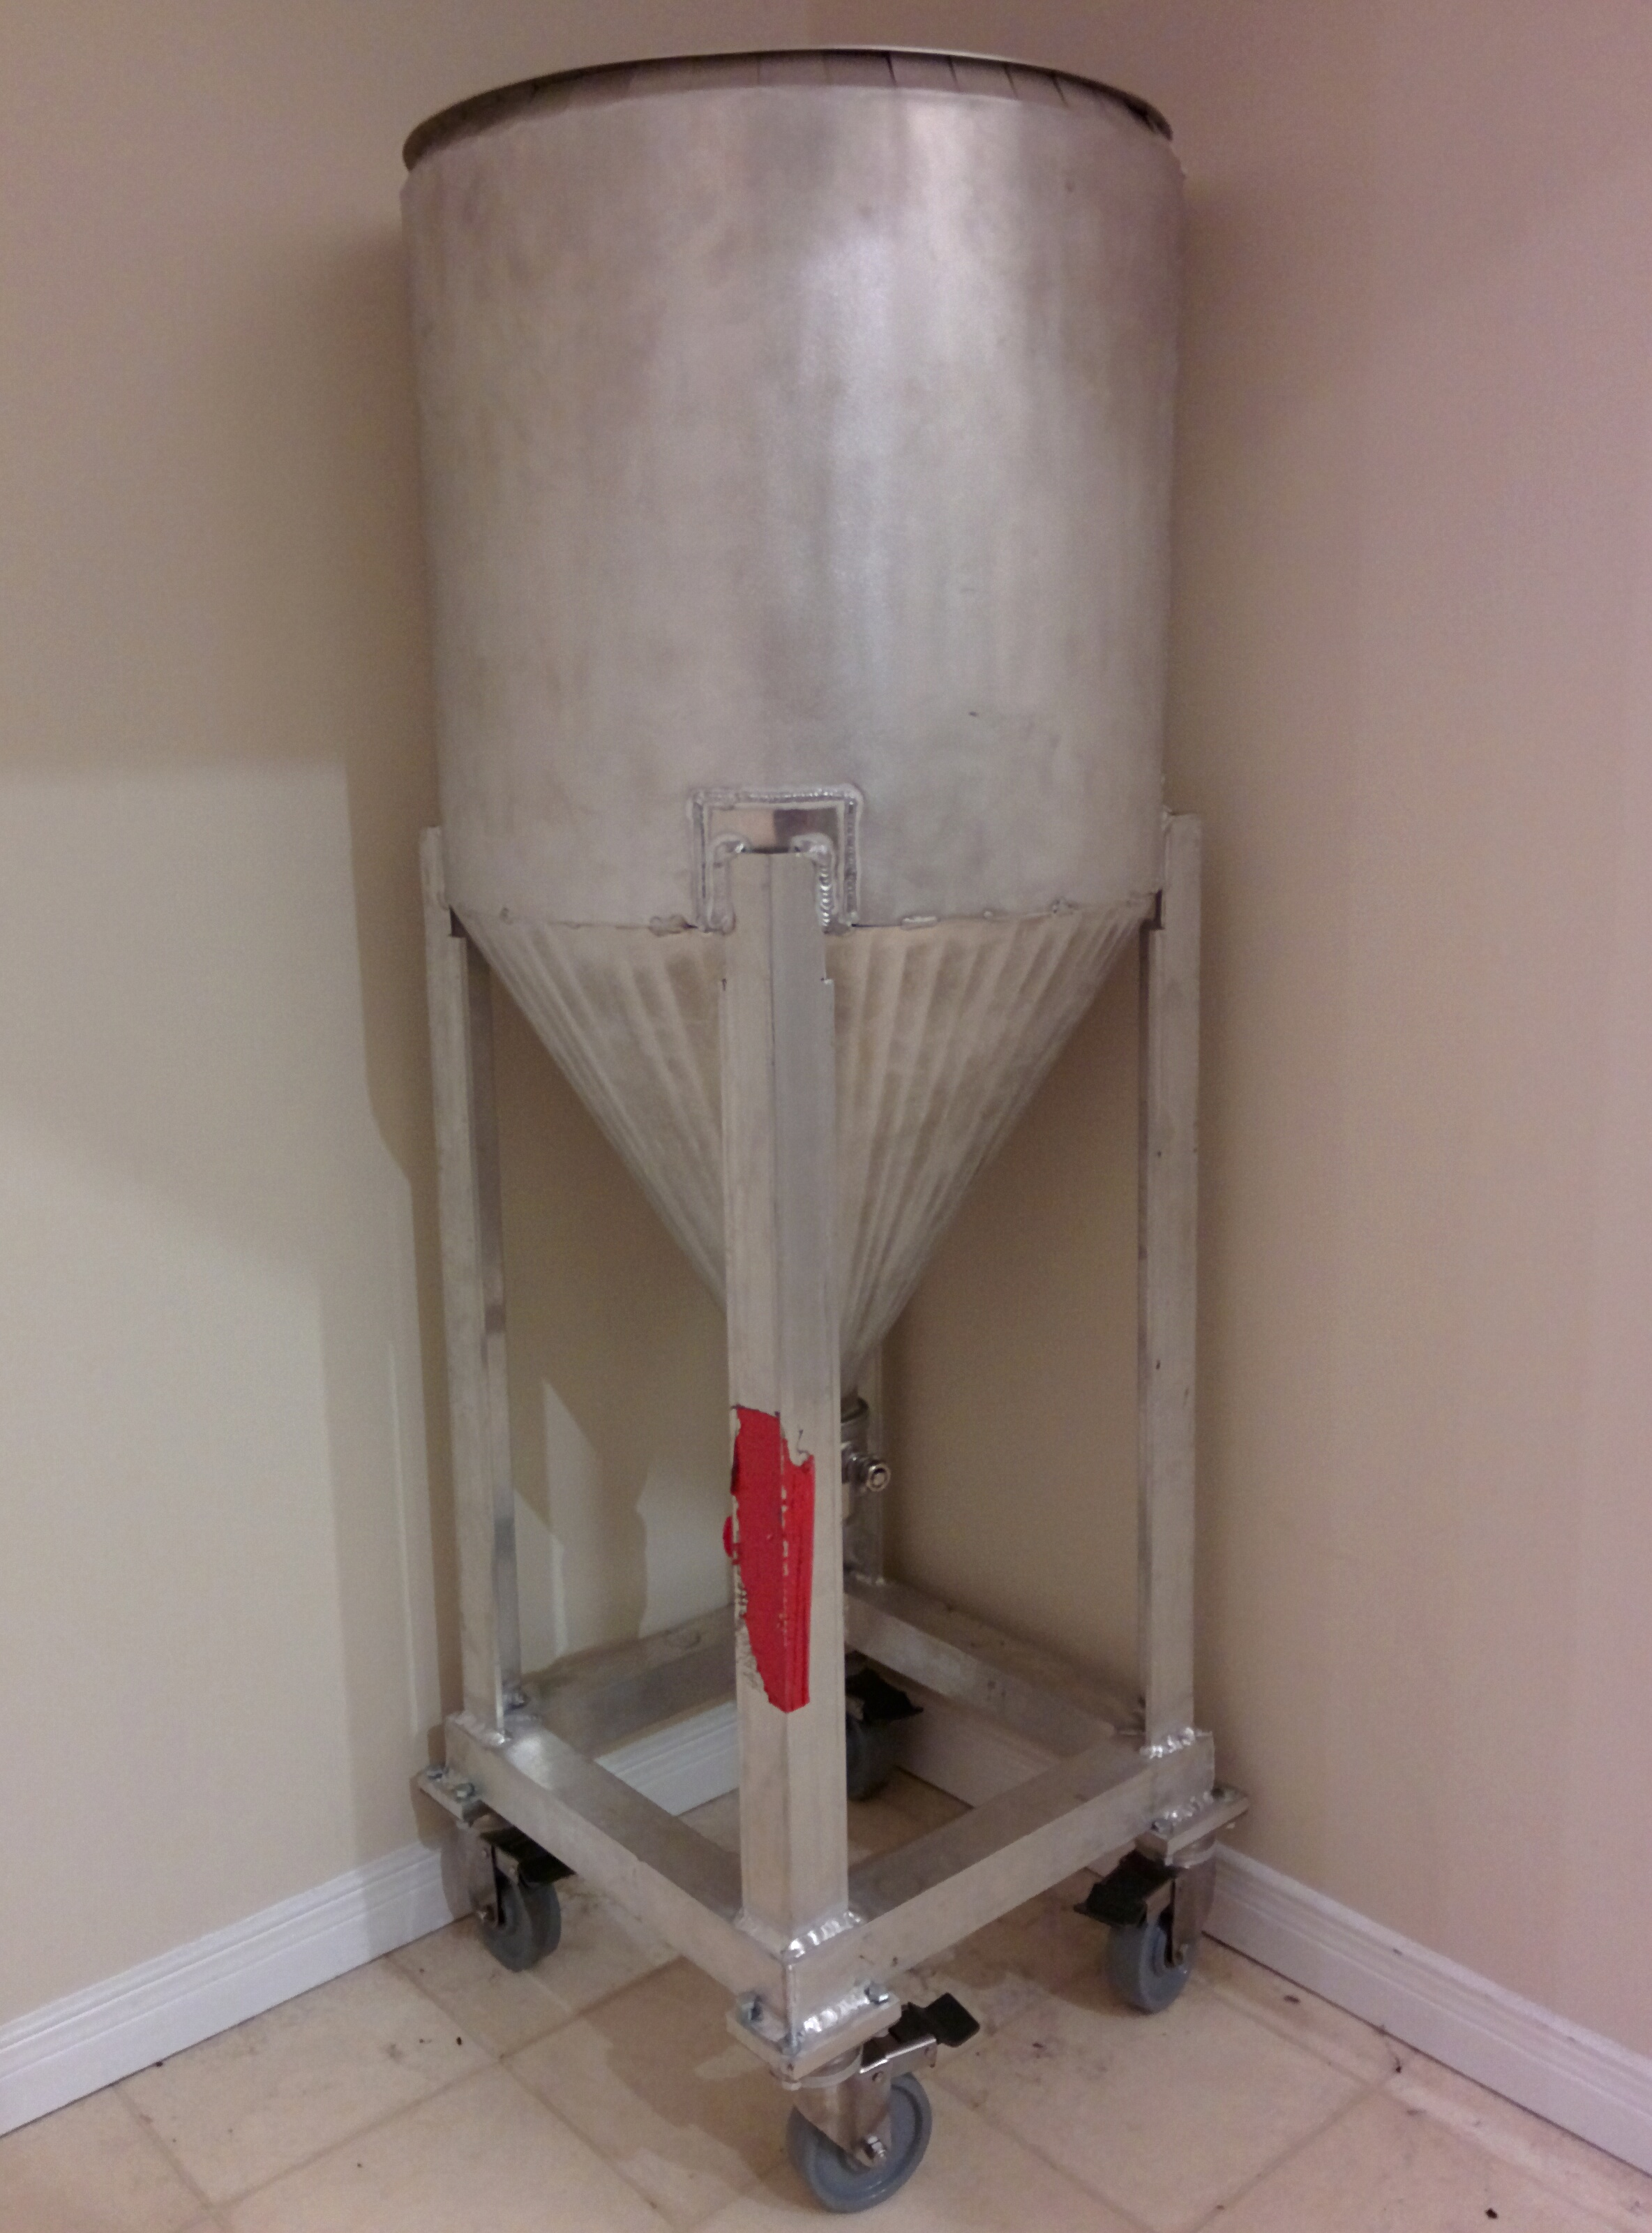
\includegraphics[scale=0.10]{mechanical-prototype.jpg}
\caption{A front view of the mechanical design of the conical fermenter}
\label{fig:mechanical-prototype}
\end{center}
\end{figure}

\subsection{Electrical System}
The electrical system consists of two main parts, the controller and the power electronic circuitry. These two subsystems are coupled closely together in that the control signals produced by the controller are amplified by the power electronics and sent to each plant. The main plants that are controlled and powered by the electrical systems are the heating element, cooling system, mixing motor, and various small similar actuators.
\subsubsection{Controller Designs}
Of the four controllable subsystems, the heating and cooling for fine temperature regulation is the highest priority for robust design. The pump and actuators are necessary for the final realised system, but can easily be constructed with off-the-shelf components and minimal design effort.
\noindent The actuators used in the system to open/close various valves and chutes are implemented using servomotors as the electrical component. The controllers used to control these actuations outputs a simple on-off signal and does not require feedback in the form of sensors.
\noindent The continuous-time transfer function model of a DC motor with motor voltage as input and gear angle as output is shown Equation \ref{eq:gear-angle}

\begin{equation}
P(s) = \frac{K}{s(\tau s + 1)}
\label{eq:gear-angle}
\end{equation}

\noindent Which is open-loop unstable when tracking a step input. However, when tracking a ramp (i.e. a constant velocity) the system is stable, though with large steady-state error. This makes intuitive sense because when a constant voltage is applied to a DC motor, the speed of the motor stabilizes to a constant value but the position of the motor goes unstable and increases indefinitely. Because of the fact that we don't require any sort of motor position tracking, nor do we require precise speed control, the control system for the pump motor is an open-loop system without any feedback. Instead, the gear ratio of the gearbox that is powered by this motor is constructed to allow us crude speed control by simply changing the voltage output to the motor.

\noindent Since the temperature model of the main volume of water is the same regardless of increasing or decreasing temperature, with only a sign-change to account for, the cooling system is assumed to function identically to the heating system in terms of power delivered to or taken from the water. Figure \ref{fig:heat-system-diagram} shows a sketch of the physical system, and the equation that relates heat input to heat storage and heat loss is described in Figure \ref{eq:heat-system}.

\begin{equation}
Qh = Qs + Ql
\label{eq:heat-system}
\end{equation}

\begin{figure}[H]
\begin{center}
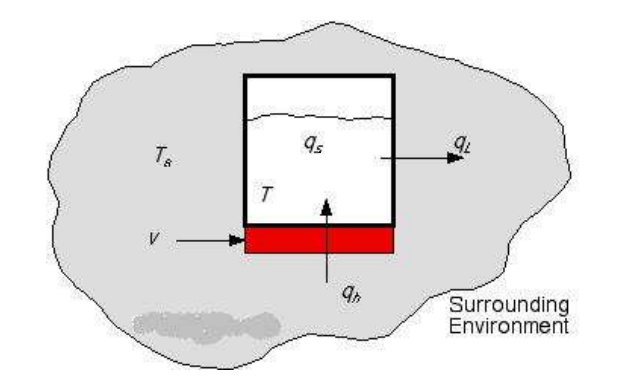
\includegraphics[scale=0.50]{heat-system-diagram.png}
\caption{A heat system diagram for a closed volume of liquid \cite{heat-modelling}}
\label{fig:heat-system-diagram}
\end{center}
\end{figure}

\noindent If we differentiate with respect to time, we get Equation \ref{eq:dt} \cite{heat-modelling}.
\begin{equation}
P = C \times \frac{dT}{dt} + k(T - T_{a})
\label{eq:dt}
\end{equation}
\noindent Where $P$ is the power input into the system, $C$ is the thermal capacity of the water, $k$ is the thermal conductance of the tank, $T_{a}$ is the ambient temperature of the room, $T$ is the temperature of the water, and t is time. Taking the Laplace transform of both side, we get Equation \ref{eq:laplace-heat}.

\begin{equation}
P(s) = C \times s \times T(s) + kT(s)
\label{eq:laplace-heat}
\end{equation}

\noindent Resulting in Equation \ref{eq:result-heat}

\begin{equation}
\frac{T(s)}{P(s)} = \frac{1}{Cs + k}
\label{eq:result-heat}
\end{equation}

\noindent Our transfer function model of the heating of a volume of liquid. Finding the value of the parameter C is relatively straightforward, it is equal to the mass of water in the system multiplied by the specific heat capacity of water. Since our system is designed to hold 50L of water, we get the result shown in \ref{eq:value-heat}

\begin{equation}
C = 50L \times 1\frac{kg}{L} \times 4200\frac{J}{kgK} = 210,000\frac{J}{K}
\label{eq:value-heat}
\end{equation}

\noindent Since the inner tank of our conical vessel is well insulated, we know that the value of $k$ (in units of Watts per Kelvin) is small. However, calculating $k$ mathematically is difficult and it is easier to instead perform some system identification on the completed system.
The controller used to control the temperature of the volume of water can be implemented in many different ways, however we are deciding to look at 2 main options: a \gls{pid} controller, and a hysteresis-thermostat controller. Pictured below in Figure \ref{fig:hysteresis-block-diagram} and Figure \ref{fig:pid-block-diagram} are Simulink models created in MATLAB to simulate these two possible controller schemes. Additionally, the tuned \gls{pid} parameters used in the latter diagram, as calculated using the built-in Simulink \gls{pid} Tuner tool-kit, are listed in Figure \ref{fig:pid-parameters}.

\begin{figure}[H]
\begin{center}
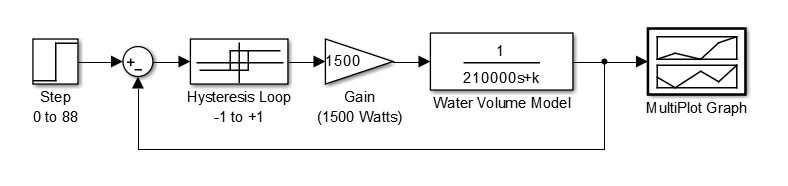
\includegraphics[scale=0.70]{hysteresis-block-diagram.png}
\caption{Hysterisis loop temperature controller and plant model}
\label{fig:hysteresis-block-diagram}
\end{center}
\end{figure}

\begin{figure}[H]
\begin{center}
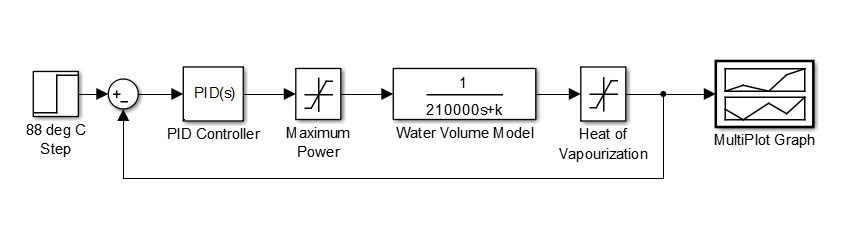
\includegraphics[scale=0.70]{pid-block-diagram.png}
\caption{\gls{pid} temperature controller and plant model}
\label{fig:pid-block-diagram}
\end{center}
\end{figure}

\begin{figure}[H]
\begin{center}
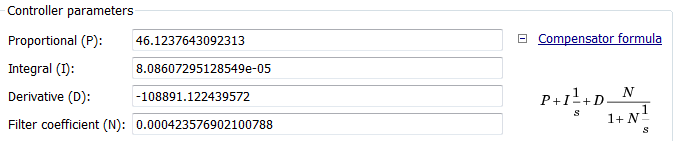
\includegraphics[scale=0.80]{pid-parameters.png}
\caption{\gls{pid} controller parameters}
\label{fig:pid-parameters}
\end{center}
\end{figure}

In these models, the step input has an amplitude of 88 degrees Celsius, simulating the heating of water from 10$^{\circ}$C to 98$^{\circ}$C; and the maximum allowable control signal is 1500W, which equates to 12.5A on standard 120V household power. We are looking to optimise a number of parameters with the selection of one of these control systems. Specifically, we want the best combination of settling time and steady-state error versus cost and complexity of implementation. Pictured below in Figure \ref{fig:hysteresis-step-lossless} and Figure \ref{fig:pid-step-lossless} are the step responses of each of these systems, simulated assuming a k-value of zero (well insulated, lossless vessel).

\begin{figure}[H]
\begin{center}
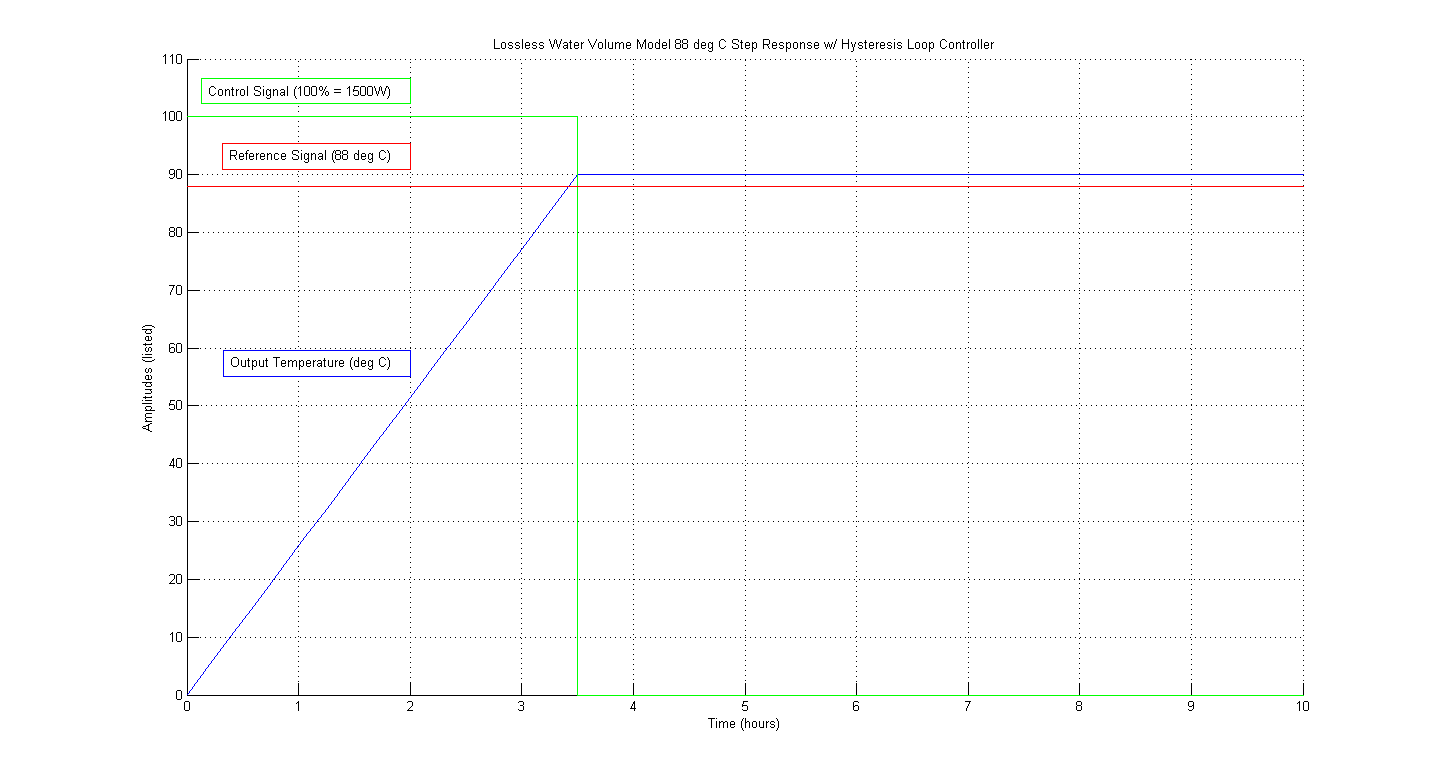
\includegraphics[scale=0.35]{hysteresis-step-lossless.png}
\caption{Lossless hysteresis loop control step response with control signal}
\label{fig:hysteresis-step-lossless}
\end{center}
\end{figure}

\begin{figure}[H]
\begin{center}
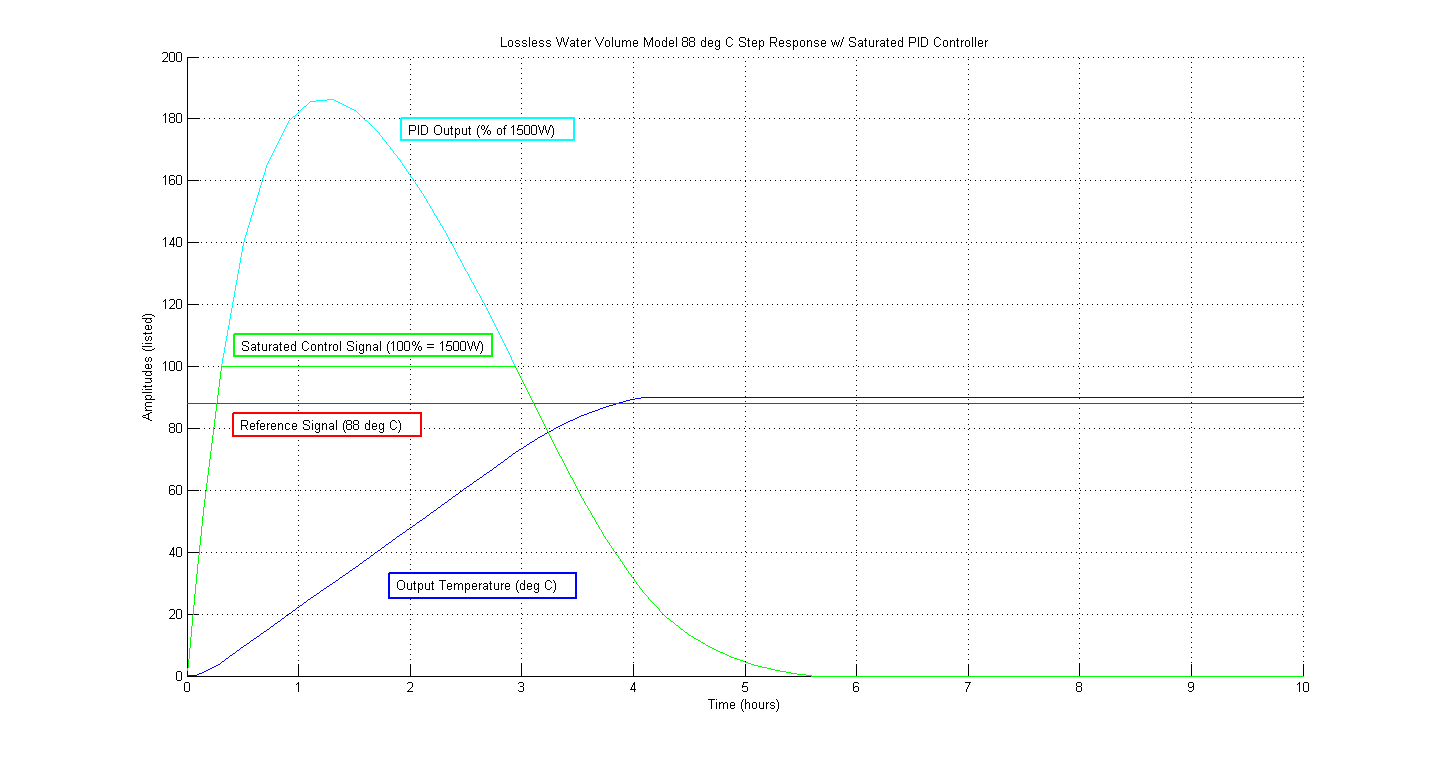
\includegraphics[scale=0.35]{pid-step-lossless.png}
\caption{Lossless \gls{pid} control step response with control signal}
\label{fig:pid-step-lossless}
\end{center}
\end{figure}

\noindent It can be seen from these plots that the hysteresis controller reaches the full-value thirty minutes earlier than the saturated \gls{pid} controller. Since this model is perfect and lossless, the operation of the hysteresis loop isn't very apparent. If we increase the thermal conduction value to a modest level (k = 10), we get the response plotted in Figure \ref{fig:hysteresis-step-lossy}. In this figure, we can clearly see that the switching period is around 20-minutes, which is long enough to ensure that we aren't over-switching our relays to run this controller. The new settling time is close to five hours in this plot.

\begin{figure}[H]
\begin{center}
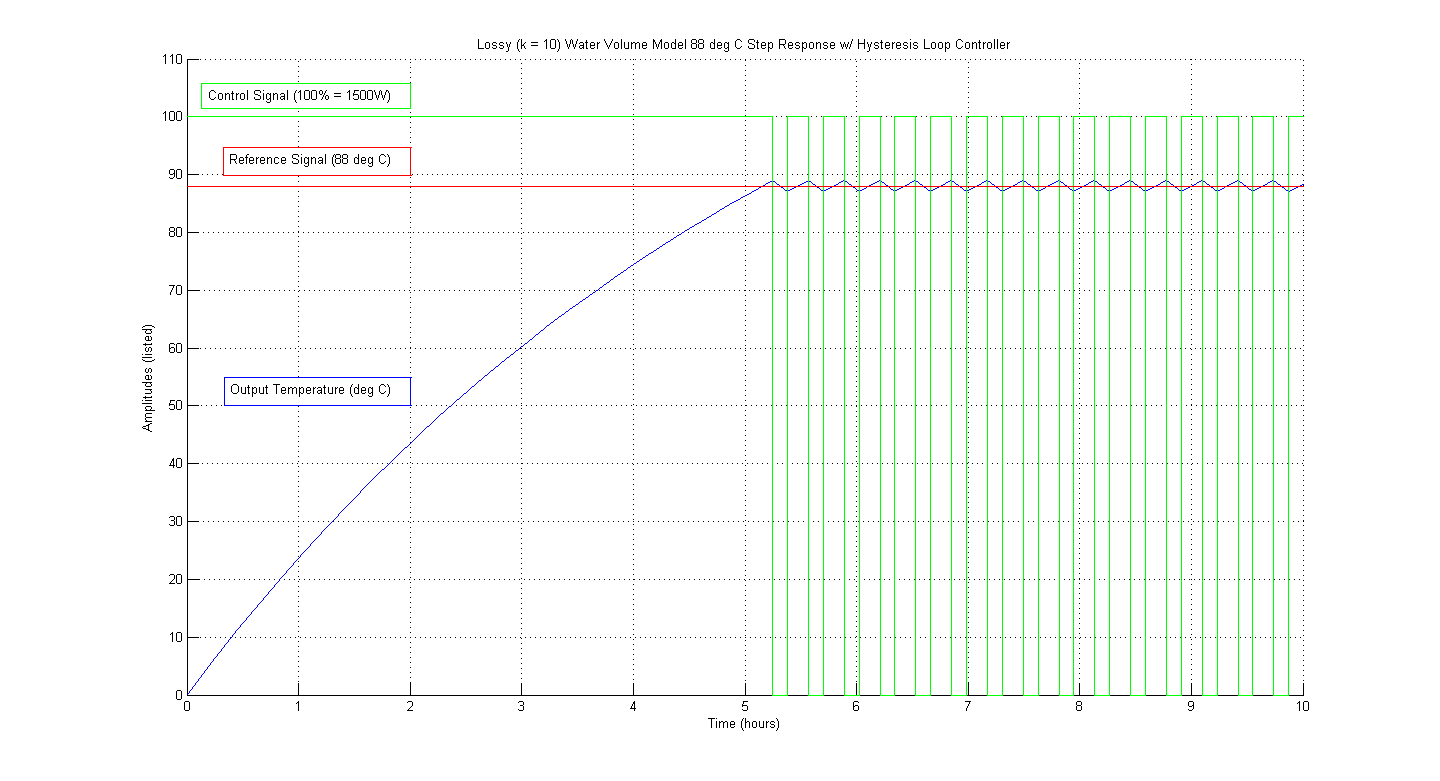
\includegraphics[scale=0.35]{hysteresis-step-lossy.png}
\caption{Lossy hysteresis loop step response with control signal}
\label{fig:hysteresis-step-lossy}
\end{center}
\end{figure}

\noindent We can compare this to Figure \ref{fig:pid-steps-various-k} which plots the response of the \gls{pid} system with varying k-values. In this plot, we see that for many values of k, the response time is also close to 5 hours, but as $k$ increases the steady-state error quickly worsens to an unacceptable level.

\begin{figure}[H]
\begin{center}
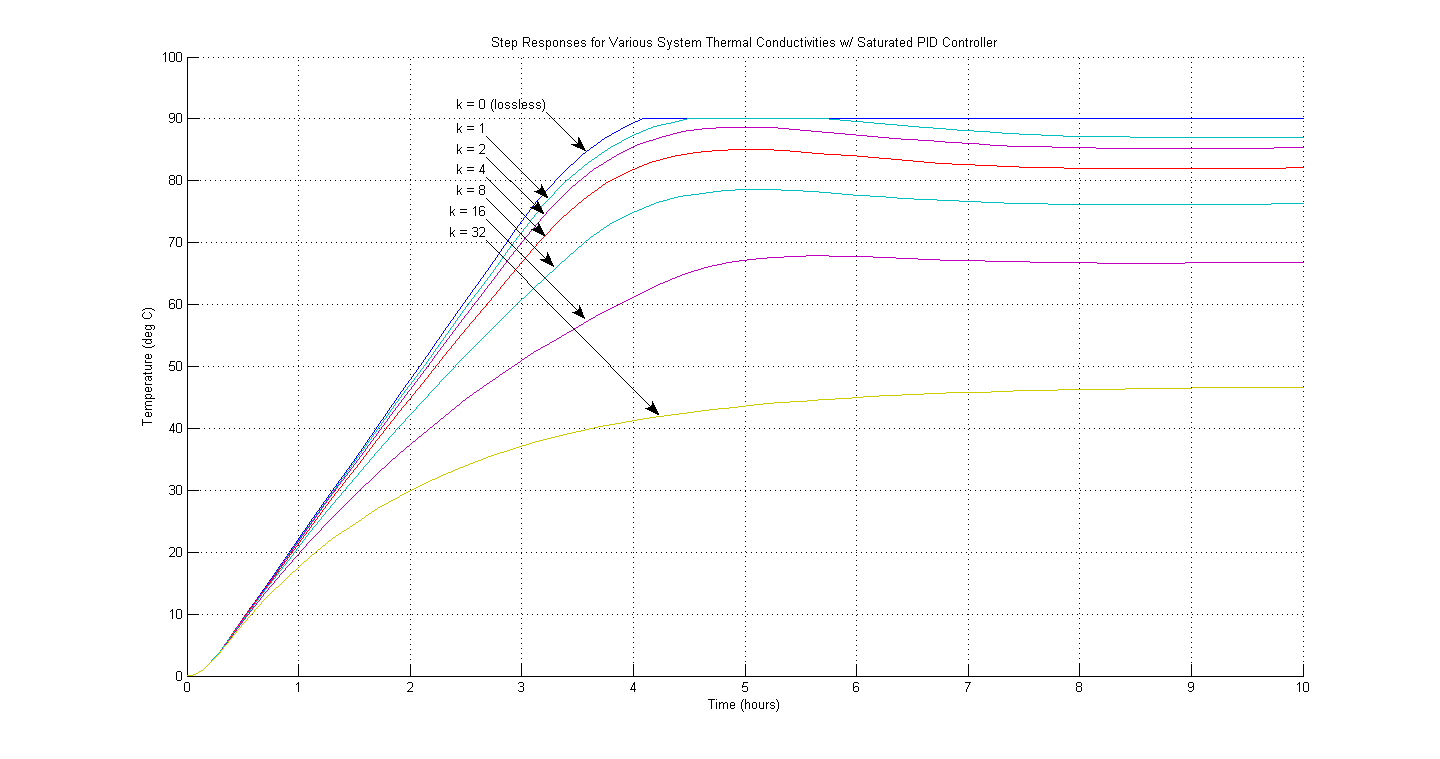
\includegraphics[scale=0.35]{pid-steps-various-k.png}
\caption{\gls{pid} controller step response for various thermal conductivities}
\label{fig:pid-steps-various-k}
\end{center}
\end{figure}

\noindent For the \gls{pid} system, the ``critical k-value", defined as the k-value for which the steady-state error is beyond an acceptable level, is below $k$ = 4. If we compare this to Figure \ref{fig:hysteresis-step-critical} where the critical k-value of 16.67 for the hysteresis controller is plotted, we can see that the hysteresis controller is much more robust when faced with uncertain values of $k$ since the critical value is over four times larger.

\begin{figure}[H]
\begin{center}
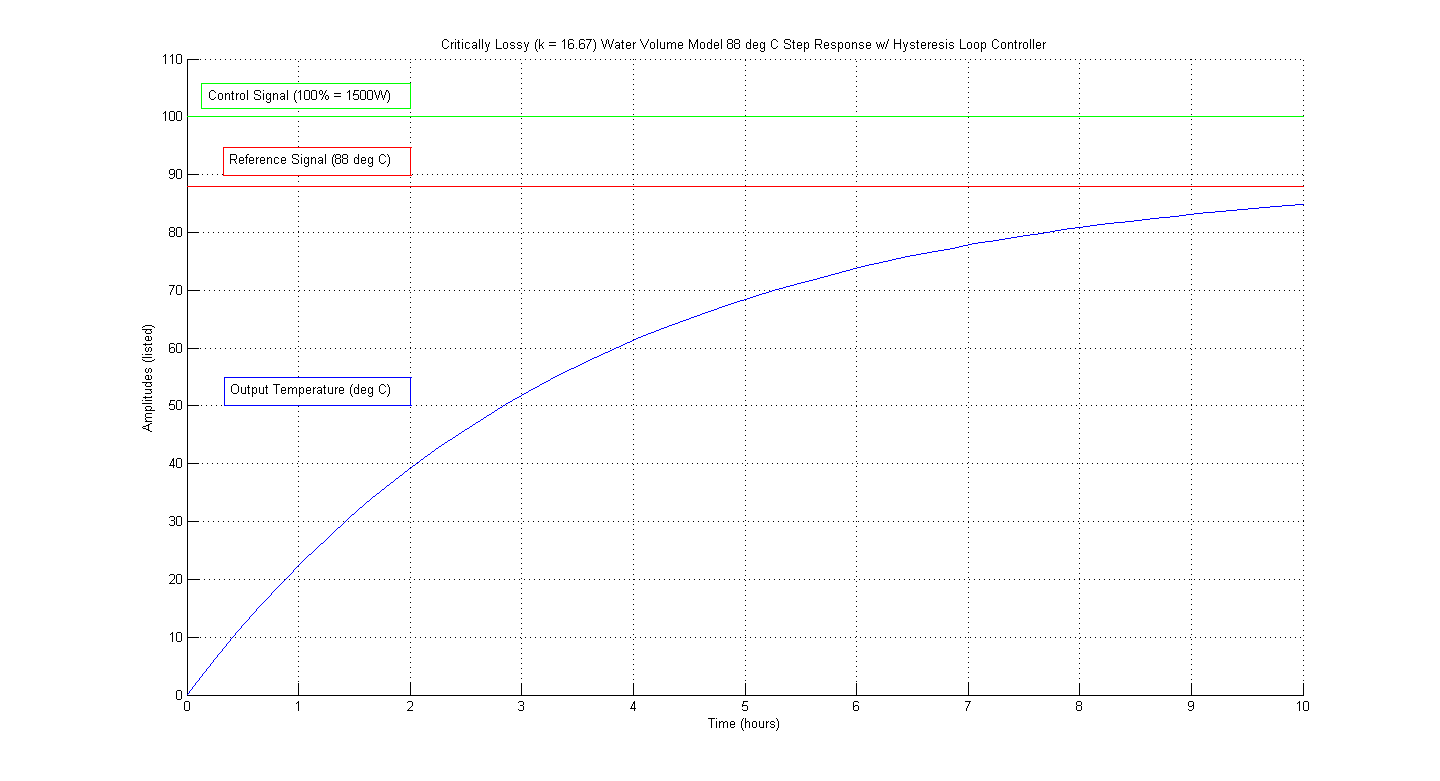
\includegraphics[scale=0.35]{hysteresis-step-critical.png}
\caption{Critically lossy hysteresis loop step response with control signal}
\label{fig:hysteresis-step-critical}
\end{center}
\end{figure}

\noindent As such, the hysteresis-loop thermostat controller is being chosen to implement the heating and cooling of the vessel. Additional to the superior performance, the hysteresis controller has the added benefit of reduced implementation complexity in terms of the required power electronic circuitry, as discussed in the next section.

\subsubsection{Power Electronics Design}
The purpose behind the design of the power electronic circuitry is to be able to effectively implement the control strategies required to meet our design criteria. With the chosen control systems discussed in the previous section, the basic design of the power electronic circuits is straightforward. Depending on the size and power requirements of the servomotors needed to actuate the mechanical chutes and valves of the system, one of two circuits can be implemented. For large servos, the circuit pictured in Figure \ref{fig:servo-large-actuator-circuit} can be implemented to power the motor.

\begin{figure}[H]
\begin{center}
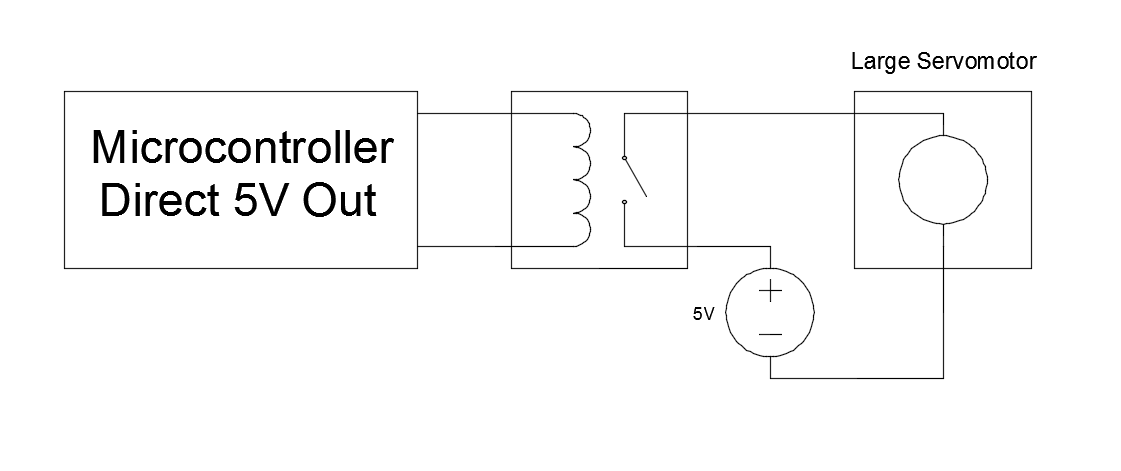
\includegraphics[scale=0.40]{servo-large-actuator-circuit.png}
\caption{Large Servo Motor Power Circuit}
\label{fig:servo-large-actuator-circuit}
\end{center}
\end{figure}

\noindent However, for smaller servos that require less current to function, the relay and external DC source can be removed from the circuit completely, and the motor can be powered directly from the microcontroller's 5V output pins, as depicted in Figure \ref{fig:servo-small-actuator-circuit}.

\begin{figure}[H]
\begin{center}
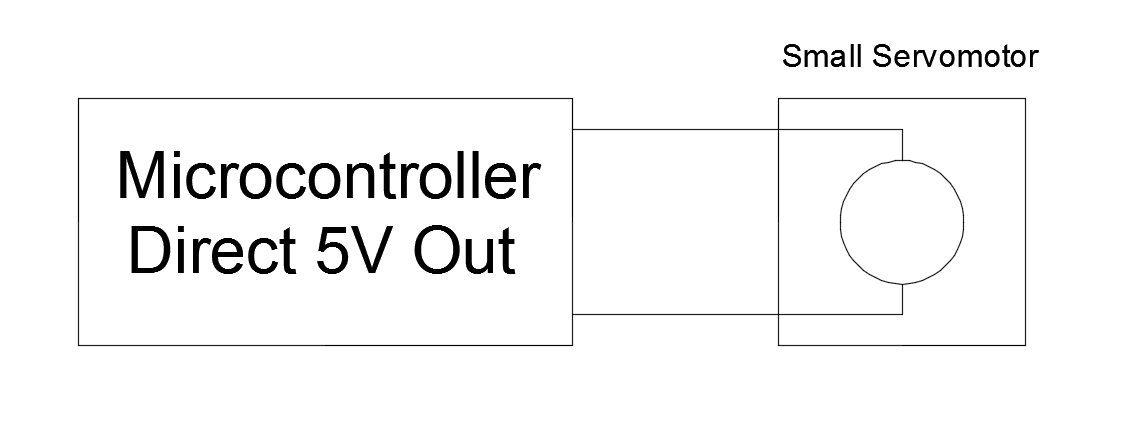
\includegraphics[scale=0.30]{servo-small-actuator-circuit.png}
\caption{Small Servo Motor Power Circuit}
\label{fig:servo-small-actuator-circuit}
\end{center}
\end{figure}

\noindent The heating element alluded to in the previous section is realised through the use of immersion hot water tank heaters. The original design called for a length of insulated resistive wire wrapped around the vessel, but that became too difficult to source parts for and implement. Additionally, the original design for the cooling system revolved around a compressor-driven refrigeration cycle with coolant coils wrapped around the vessel walls, but once again the sourcing of a refrigeration system proved too difficult to implement. Instead, the cooling is realised by an array of 20 solid-state Peltier cooling tiles scattered evenly around the vessel walls. Heat from the hot side of the tiles will be sunk away via aluminum blocks with water channels, where water passes through them to an outer reservoir with a larger forced-air heat sink. The Peltier tiles are powered through a purchased 12V, 1500W supply with a relay on the 120V input such that the control circuitry becomes identical to the heater.

\noindent Figure \ref{fig:heater-hysteresis-circuit} and Figure \ref{fig:heater-pid-circuit} illustrate the circuits for the hysteresis control and the unselected \gls{pid} control schemes respectively. The Hysteresis control is realised with a simple circuit consisting of a relay between the 120V power supplied by the house and the immersion heating element. The \gls{pid} controller could have been realised with a triac whose firing angle is varied to modulate the power output to the heating coil.

\begin{figure}[H]
\begin{center}
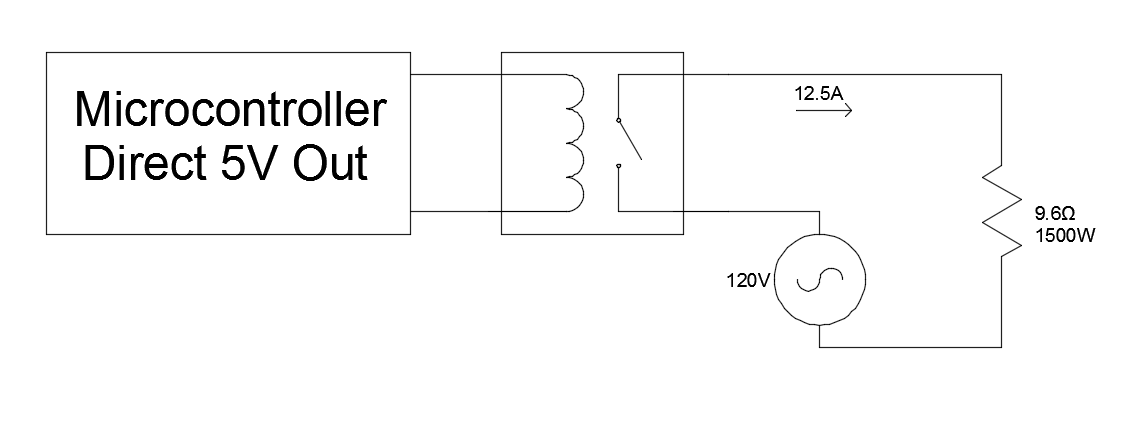
\includegraphics[scale=0.40]{heater-hysteresis-circuit.png}
\caption{Hysteresis Loop Controller Power Circuit}
\label{fig:heater-hysteresis-circuit}
\end{center}
\end{figure}

\begin{figure}[H]
\begin{center}
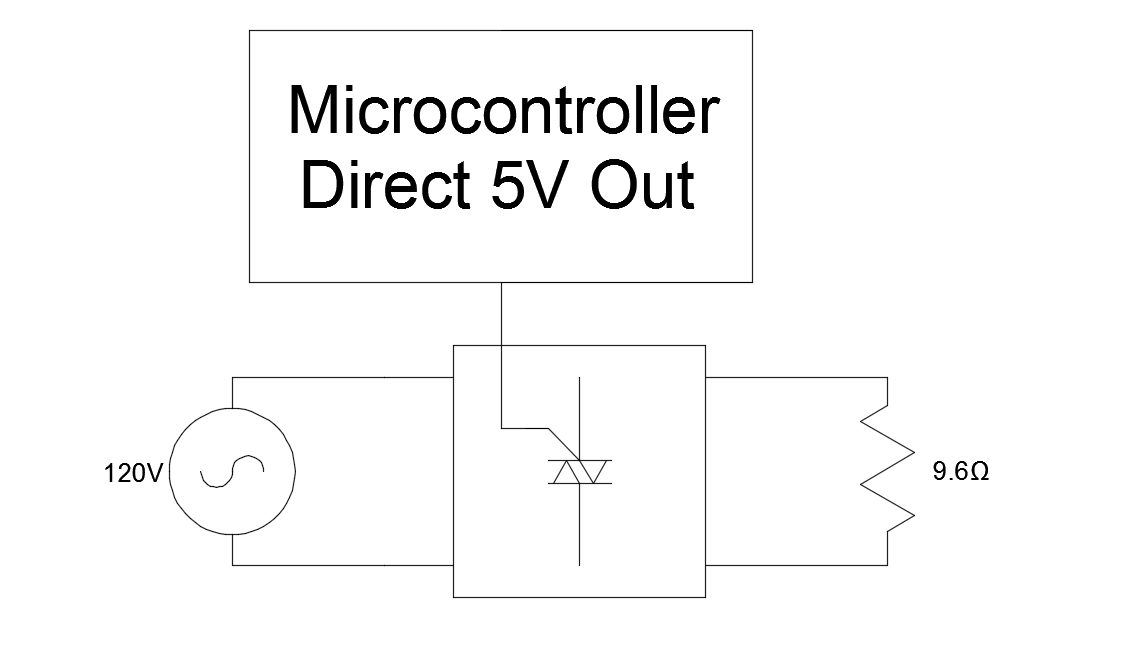
\includegraphics[scale=0.30]{heater-pid-circuit.png}
\caption{\gls{pid} Controller Power Circuit}
\label{fig:heater-pid-circuit}
\end{center}
\end{figure}

\noindent The pumping system is driven by a DC motor, and the circuit used to power it is pictured in Figure \ref{fig:motor-thyristor-dc-circuit}. It consists of a step-down transformer to reduce the mains voltage down to 12 volts to power the motors, then a full-bridge thyristor rectifier is used to simultaneously rectify the AC input voltage to a DC voltage and control the magnitude of the output voltage by varying the thyristor firing angle α. The DC motor can be modeled as an inductance in series with a resistance, followed by a reverse-emf voltage.

\noindent The original design called for an additional large DC motor to power a mechanical mixer that would be submersed in the vessel, however it was decided that the turbulence generated from boiling would suffice to aid in the extraction of sugars from the grain.

\begin{figure}[H]
\begin{center}
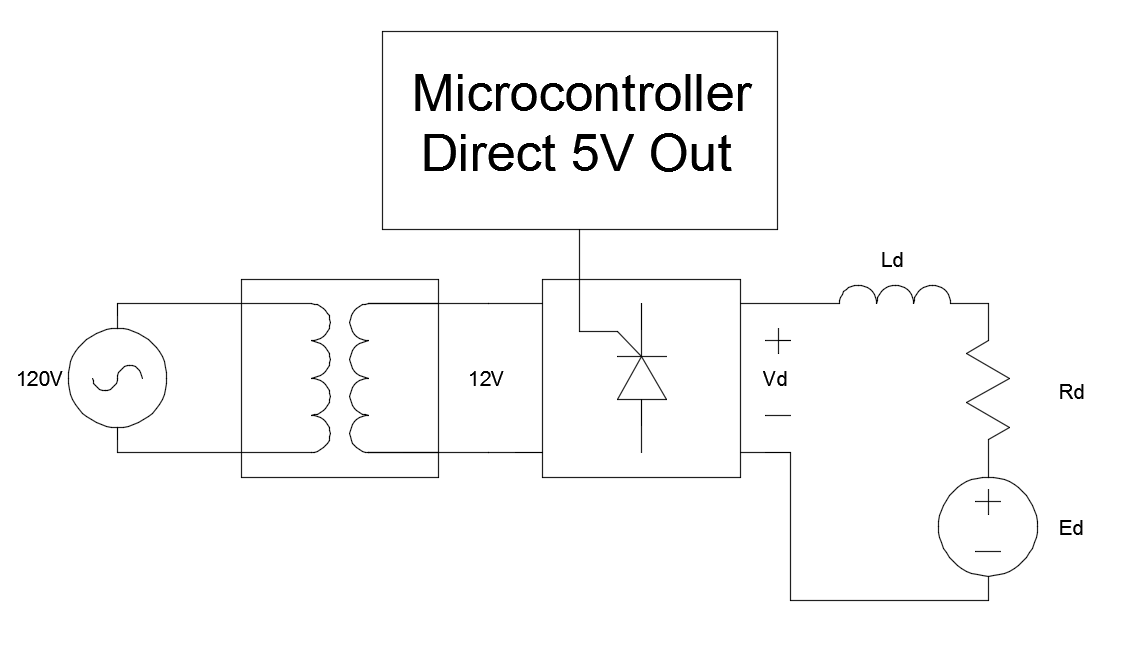
\includegraphics[scale=0.40]{motor-thyristor-dc-circuit.png}
\caption{Thyristor Bridge Motor Power Circuit}
\label{fig:motor-thyristor-dc-circuit}
\end{center}
\end{figure}

\subsubsection{Prototype Circuitry}
Since we only recently received our vessel back from the machine shop from welding, none of the test electronics have been installed. However, Figure \ref{fig:electrical-prototype} shows a test board where the relays have been tested by powering loads, controlled by the microcontroller on the far right. The next step is to install these components and their duplicates into a NEMA-rated electrical box, affix the actuatable components to the vessel, and run the wiring between everything.

\begin{figure}[H]
\begin{center}
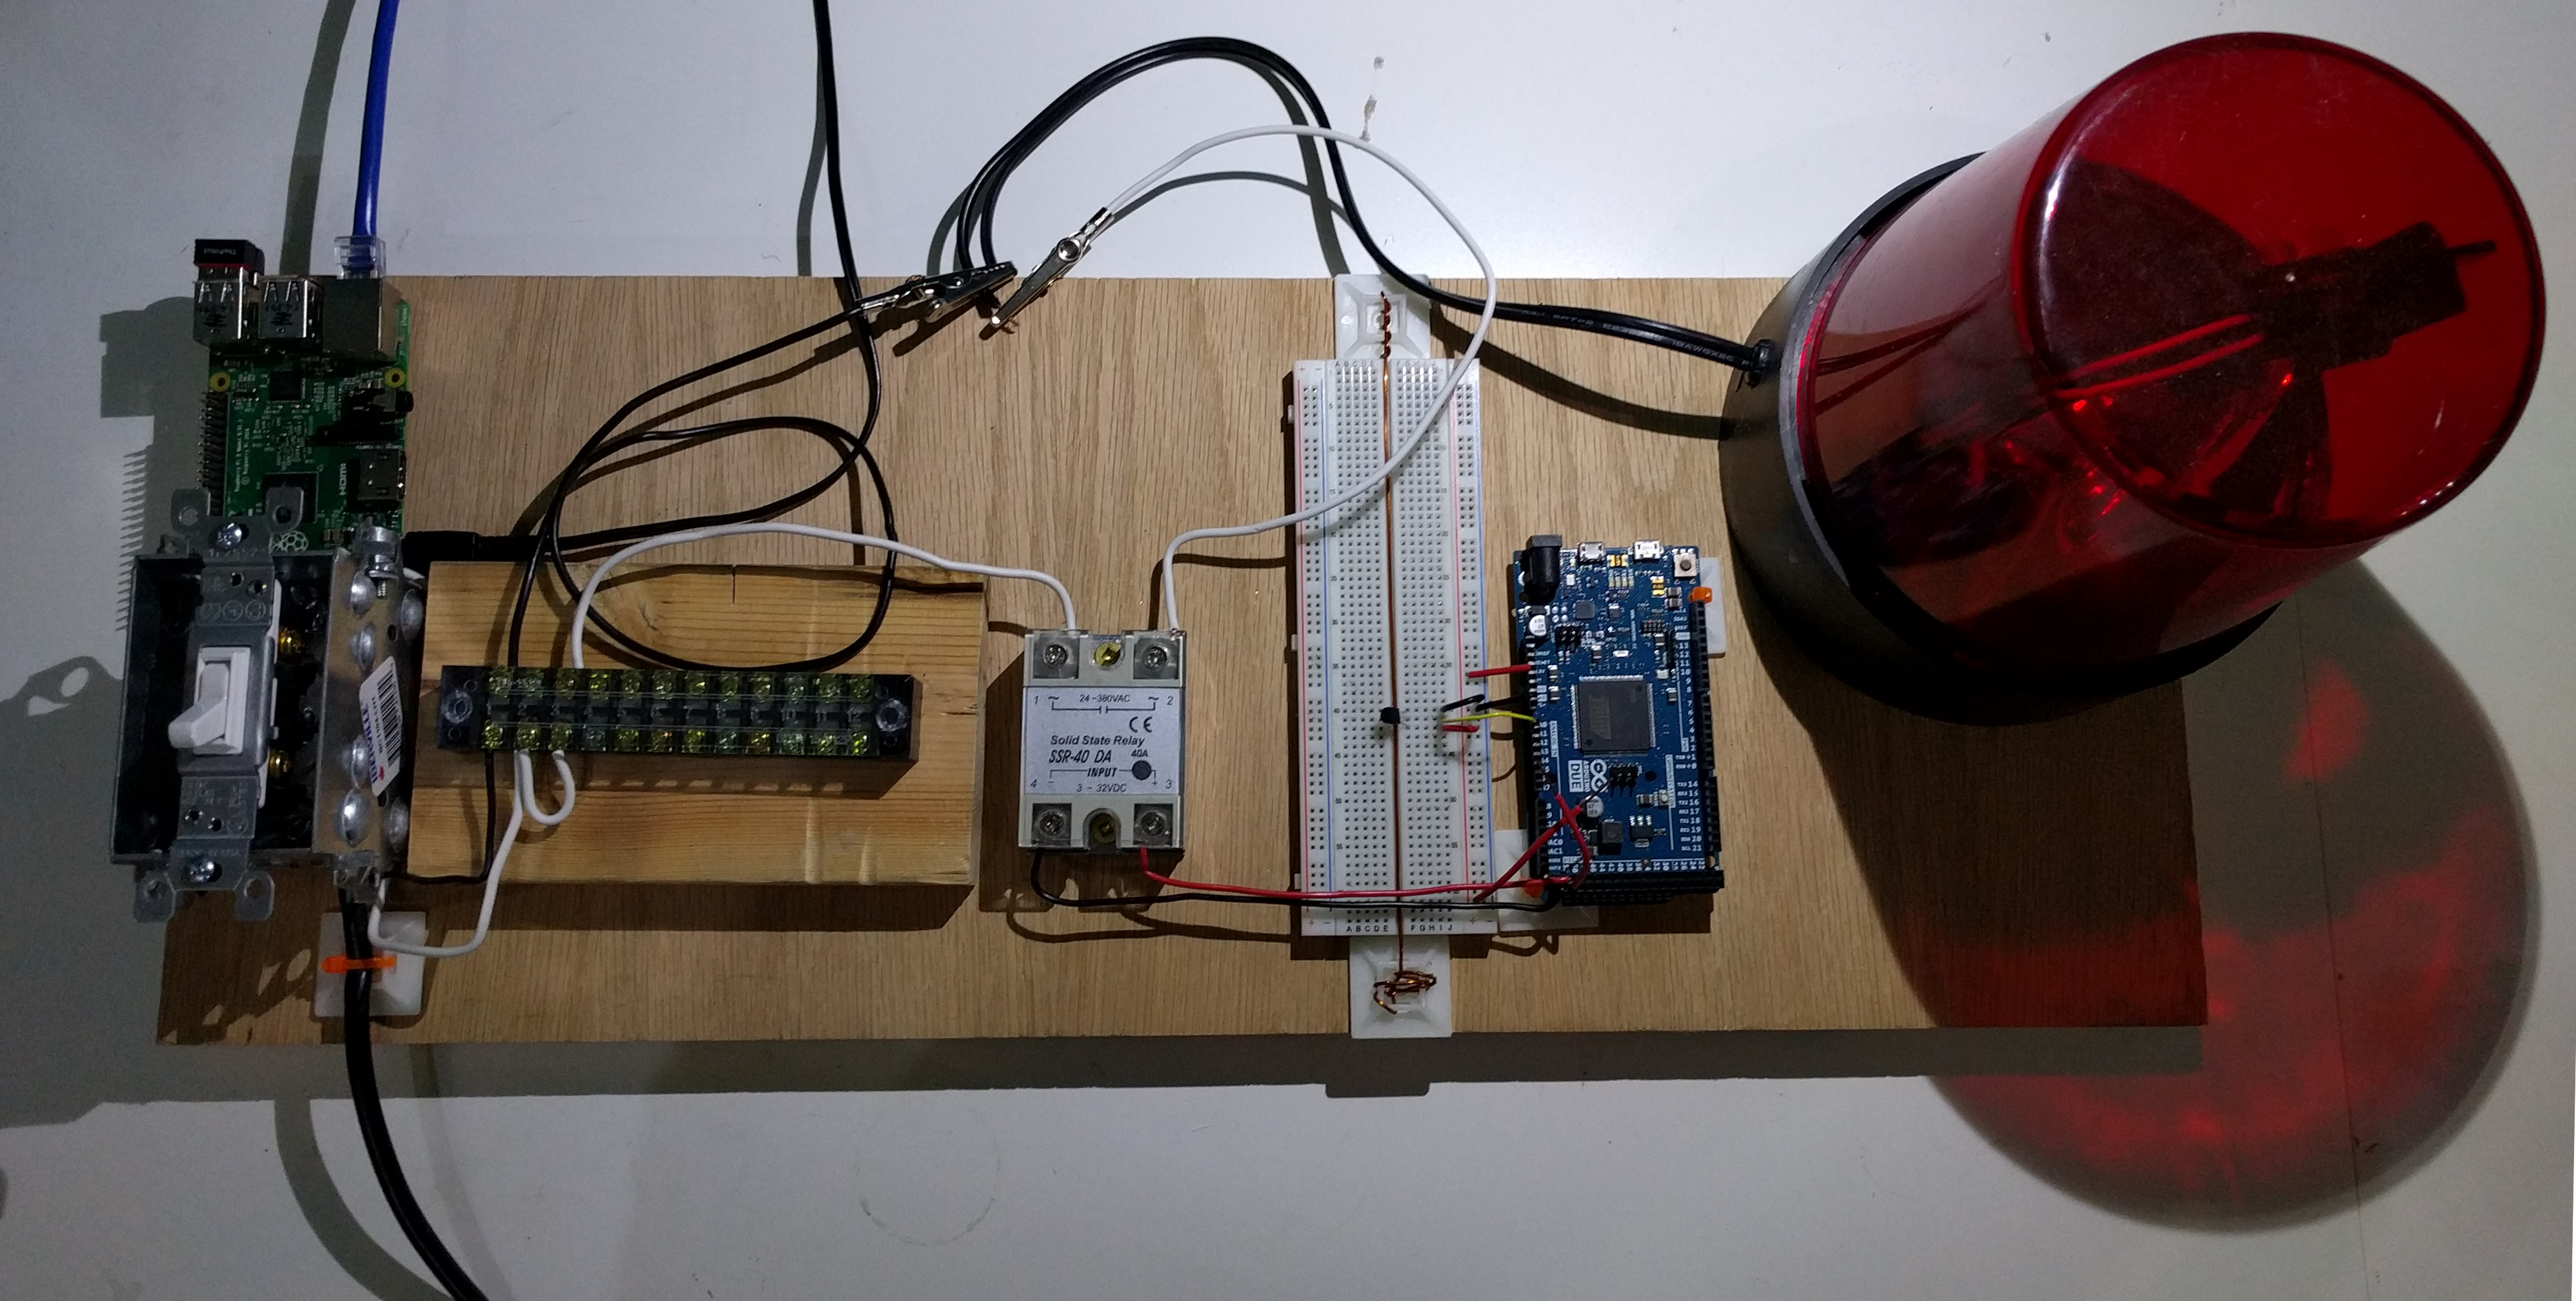
\includegraphics[scale=0.1]{electrical-prototype.jpg}
\caption{Electrical Prototype}
\label{fig:electrical-prototype}
\end{center}
\end{figure}

\subsection{Computer System}
The computer systems consist of three main components, the embedded central computer, the microcontroller and sensor pairs, as well as a Web Server and Database pair to allow for storage and communications.  The detailed description of each subcomponent and the methods of interaction between them is discussed in this section.
\subsubsection{Embedded Computer}
The primary function of the embedded computer system is to aggregate data in close to real-time from the multiple sensors used in the design.  Analysis of this data is crucial for determining the current progress in the \gls{mash}, \gls{sparge}, and boiling of the \gls{wort}.  For specific analysis of sensor data please see subsection \ref{subsec:sensor}.

For ease of repeatability, availability, and cost the \gls{rpi} was selected.  At the time of design and creation of this report, this is the most recent hardware revision of the \gls{rpi}.  The relevant hardware specifications for the \gls{rpi} is a quad-core \gls{arm} processor, 1GB of \gls{ram}, and a Bluetooth dongle for local wireless communications (rated to 50m).  Since the outer shell of the fermenter is aluminum, the casing for the \gls{rpi} can act as a heat sink, allowing it to be safely overclocked to 1GHz, 500MHz, and 500MHz for the \gls{arm} processor frequency, sdram frequency, and L2 cache (core) frequency respectively.  The configuration file below allows for a substantial performance boost with negligible thermal impact.  

\begin{lstlisting}
arm_freq=1000
sdram_freq=500
core_freq=500
over_voltage=2
arm_freq_min=400
sdram_freq_min=250
core_freq_min=250
\end{lstlisting}

The operating system chosen was the \gls{arm} build of Ubuntu 14.04 \gls{lts}, codename Trusty Tahr, as well as \gls{ros} Jade Turtle for sensor coordination and communication.  Ubuntu 14.04 was chosen over the default Raspbian operating system for increased security due to the use of SELinux policies.  Since the \gls{rpi} will be acting as a \gls{lamp} server as well for mobile interaction and remote notifications, enforcing read only access over the configured port of choice is a necessity. For an in depth overview of the mobile application please see subsection \ref{subsec:mobile-app}.  Additionally, the \gls{lts} version of Ubuntu was chosen for a maximum of five years support, as well as increased compatibility and reliability for repository packages specific to the trusty distribution.

\subsubsection{Sensors and Microcontrollers}\label{subsec:sensor}
Every sensor in the system is paired with a microcontroller to enable a modular design and a plug and play like support.  By adding more sensors to the system, more information can be provided as feedback to enable better logging and regulation of the brewing environment.  The only mandatory sensors for the system are a main temperature sensor for the \gls{wort} and flow meters on the liquid inputs and outputs of the system.  By introducing additional sensors, such as pH and density sensors, certain yield thresholds of interest in the \gls{sparge} and fermentation procedure can be met rather than approximated.  Additionally, this will allow for a tier based configuration for the automated vessel to reduce cost and complexity if desired.  As the end goal for this project is to have a community influenced input, having a customizable sensor configuration with open hardware and software pairs is encouraged.  For maximum affordability the Arduino compatible Teensy-LC microcontroller is used to poll the sensors and report data, however any Arduino compatible microcontroller may be used. The bridge between the \gls{ros} instance on the \gls{rpi} and the Arduino compatible microcontroller is achieved through the use of the ROSserial package.  Example code for obtaining data from a TMP102 temperature sensor over \gls{i2c} at address 0x91 \cite{tmp102} can be seen below \cite{rosserial}.

\begin{lstlisting}
#include <Wire.h>
#include <ros.h>
#include <std_msgs/Float32.h>

//Set up the ros node and publisher
std_msgs::Float32 temp_msg;
ros::Publisher pub_temp("temperature", &temp_msg);
ros::NodeHandle nh;

int sensorAddress = 0x91 >> 1;  // From datasheet
long publisher_timer;

void setup()
{
  Wire.begin();        // join i2c bus (address optional for master)
  nh.initNode();
  nh.advertise(pub_temp);
}

void loop()
{
  if (millis() > publisher_timer) {
  // step 1: request reading from sensor
    Wire.requestFrom(sensorAddress,2);
    delay(10);
    if (2 <= Wire.available())  // if two bytes were received
    {
      byte msb;
      byte lsb;
      int temperature;

      msb = Wire.read();  // receive high byte (full degrees)
      lsb = Wire.read();  // receive low byte (fraction degrees)
      temperature = ((msb) << 4);  // MSB
      temperature |= (lsb >> 4);   // LSB

      temp_msg.data = temperature*0.0625;
      pub_temp.publish(&temp_msg);
    }
  publisher_timer = millis() + 1000; //publish once a second
  }
  nh.spinOnce();
}
\end{lstlisting}

Additionally, controllers can be linked to the system via Arduino compatible microcontrollers and receive inputs based on sensor data gathered via \gls{ros} publications.  To improve the resolution or accuracy of data and controls, the polling interval of each of the microcontrollers can be calibrated appropriately.  Since most sensors will remain idle for a majority of the brewing process, their sampling rates can be scaled using a simple algorithm as suggested in the code sample below.

\begin{lstlisting}
#include <std_msgs/Float32.h>

int sample_rate = MIN_SAMPLE_RATE;
int sample_count = 0;

void scale_rate(std_msgs::Float32 prev, std_msgs::Float32 curr)
{
    if(prev == curr)
    {
        sample_count++;
    }
    else
	{
        sample_count--;
	}

	if(sample_count == SCALE_THRESHOLD)
	{
   		sample_rate = increase_rate();
    	sample_count = SCALE_THRESHOLD >> 1;
	}
	else if(sample_count == 0)
	{
    	sample_rate = decrease_rate();
    	sample_count = SCALE_THRESHOLD >> 1;
	}
}
\end{lstlisting}

The two fundamental controllers that require communications for the operation of the system are the water controller and the heating and cooling controllers.  Figure \ref{fig:water-controller} demonstrates a state diagram for the water controller and Figure \ref{fig:temperature-controller} demonstrate the state diagrams for toggling the heating and cooling states of the temperature controller.  The variables volume, temp, target and offset represent the current volume, current temperature, desired resultant, and amount of allowed deviation from target respectively.

\begin{figure}[H]
\begin{center}
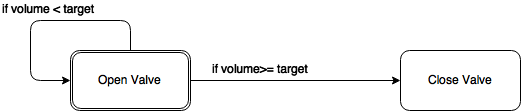
\includegraphics[scale=0.70]{water-controller-state-diagram.png}
\caption{State diagram for the water controller component}
\label{fig:water-controller}
\end{center}
\end{figure}

\begin{figure}[H]
\begin{center}
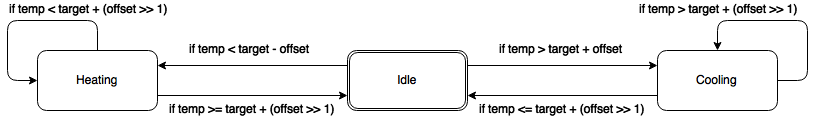
\includegraphics[scale=0.50]{temperature-controller-state-diagram.png}
\caption{State diagram for the temperature controller component}
\label{fig:temperature-controller}
\end{center}
\end{figure}

\subsubsection{Web Server and Database}
A \gls{lamp} server is the current solution for delivering information from the embedded computer to the mobile application.  All communications and parameters are to be communicated using a \gls{json} format.  The database will consist of relational connections between recipes, instructions, ingredients, sensors, and logged data as demonstrated in Figure \ref{fig:database-diagram}.

\begin{figure}[H]
\begin{center}
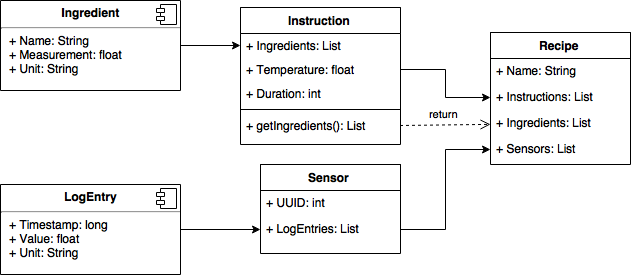
\includegraphics[scale=0.60]{database-uml-diagram.png}
\caption{A UML diagram showing the relation between tables and their entries in the logging database}
\label{fig:database-diagram}
\end{center}
\end{figure}

An important component of the web server is the server to client communication. The communication will be done through using the \gls{gcm}. This service allows a server to send messages to clients on various platforms \cite{gcm}.  There are two types of messages that can be sent using \gls{gcm}, notification and data messages. The differences between the notification and data messages is that \gls{gcm} automatically displays the notification messages on the client's behalf. Where as the data messages has to be parsed by the client in order to be used. Another difference is while the notification type messages has fixed key value pairs, data type messages can have custom ones. Both message types are in \gls{json} format, which is shown below.

\begin{lstlisting}
{
     "to" : "XYZ",
     "data" : {
     "degrees" : "85",
     "component" : "Water"
     }
}
\end{lstlisting}

The ``to" value holds the unique application id and the data block holds the key value pairs that are encapsulated in the message.
For message passing, this application uses the data message type. This is because notification messages does not offer custom key-value pairs that is required for transferring information from server to client. Although additional processing is done in the client side, data messages can be flexible to handle the various state changes that the system may undergo. In conclusion, the \gls{gcm} component of the web server uses the \gls{xmpp} protocol that sends data type messages to the client. 

\subsubsection{Sparging Algorithms}
The no-\gls{sparge} technique uses approximately 25\% more grain than a standard recipe and allows for the sparging process to be bypassed with no ill effects to the brew.  As a result, this method produces a richer, smoother-tasting \gls{wort} with the same \gls{gravity} as a standard recipe, but with a \gls{mash} and optionally a \gls{lauter} process that makes the \gls{wort} more robust and pH stable.  Not only is the end result more desirable to the consumer, but having a pH stable \gls{wort} allows for a reduced risk of souring due to bacteria and diminishes the chances of abnormal deviations.  Ultimately, this process greatly reduces the complexity of the all grain brewing process as well as the overall complexity of the system.

The following calculations combine the scaling-up of the \gls{grain-bill} with a three-step infusion-\gls{mash} that makes the whole process more manageable \cite{sparging}.  Below is a list of the relevant symbols and terms used for input parameters, constants, and output parameters respectively.

\noindent \\The input parameters to the no \gls{sparge}: \\
$OG$ is the standard recipe original \gls{gravity} \\
$G_{r}$ is the standard recipe \gls{grain-bill} \\
$V_{r}$ is the standard recipe batch size in gallons \\
$V_{b}$ is the standard recipe boil volume in gallons \\

\noindent Relevant constants to be considered: \\
$k$ is the water retention coefficient (0.125 gal/lb) \\
$R_{r}$ is the standard recipe conversion rest \gls{mash} ratio (typically 1 qt/lb) \\

\noindent The output parameters: \\
$S$ is the scale-up factor for the \gls{grain-bill} \\
$G_{n}$ is the no-\gls{sparge} \gls{grain-bill} in pounds \\
$BG$ is the no-\gls{sparge} boil \gls{gravity} \\
$R_{n}$ is the no-\gls{sparge} final \gls{mash} ratio (qt/lb) \\
$W_{n}$ is the no-\gls{sparge} total water volume in quarts \\
$W_{mo}$ is the \gls{mash}-out water volume in quarts \\
$V_{t}$ is the no-\gls{sparge} total \gls{mash} volume in quarts \\

\noindent The scale up factor is calculated by using Equation \ref{eq:scale-up} and is used in determining the no-\gls{sparge} \gls{grain-bill}.

\begin{equation}
S = \frac{V_{b}}{(V_{b} - kG_{r})}
\label{eq:scale-up}
\end{equation}

\noindent The no-\gls{sparge} \gls{grain-bill} is calculated using Equation \ref{eq:grain-bill}.

\begin{equation}
G_{n} = S \times G_{r}
\label{eq:grain-bill}
\end{equation}

\noindent The no-\gls{sparge} boil \gls{gravity} is adjusted by using Equation \ref{eq:boil-gravity}.

\begin{equation}
BG = OG \times \frac{V_{r}}{V_{b}}
\label{eq:boil-gravity}
\end{equation}

\noindent The total no-\gls{sparge} water volume in quarts is determined by Equation \ref{eq:water-volume}.

\begin{equation}
W_{n} = 4(V_{b} + kG_{n})
\label{eq:water-volume}
\end{equation}

\noindent By using Equation \ref{eq:mash-ratio} the no-\gls{sparge} \gls{mash} ratio is calculated.

\begin{equation}
R_{n} = \frac{W_{n}}{G_{n}}
\label{eq:mash-ratio}
\end{equation}

\noindent The volume of water used for the \gls{mash}-out in quarts is determined by Equation \ref{eq:water-mashout}.

\begin{equation}
W_{mo} = G_{n}(R_{n} - R_{r})
\label{eq:water-mashout}
\end{equation}

\noindent Finally, the total no-\gls{sparge} \gls{mash} volume in quarts is calculated using Equation \ref{eq:mash-volume}.  The volume of 1 pound of dry grain, mashed at 1 quart per pound, has a volume of 42 fluid ounces or 1.3125 quarts. Higher ratios only add the additional water volume, but can be used for different styles of recipes.

\begin{equation}
V_{t} = G_{n}(1.3125 + (R_{n} - 1)
\label{eq:mash-volume}
\end{equation}

By using the methods listed above, the no-\gls{sparge} process is successfully implemented while maintaining compatibility with standard recipes and the all grain brewing process.

\subsubsection{\gls{rest} Web Server}
The \gls{rest}ful Web Server is implemented using the \gls{jersey}. The \gls{jersey} provides various \glspl{api} and services to streamline web server development. Services such as \gls{json} parsing and formatting, error logging and \gls{url} mappings are all handled by this framework. There are two main functionalities that is implemented in the web server; the \textit{GCMNotificationResource} and the \textit{BrewLogResource}. Each functionality is mapped to a \gls{url} endpoint called a \gls{resource}. A sample of the \textit{GCMNotificationResource} is shown in the code sample below. The following code samples are all written in Java.

\begin{lstlisting}
@Path("gcm_notification")
public class GCMNotificationResource {

    GCMSender gcmSender;

    @GET
    @Path("/send")
    public Response sendSimpleMessage(String message) {
        GCMSender.gcmSendMessage(message);

        return Response.ok().build();
    }
}
\end{lstlisting}

\noindent The above resource is called whenever the system needs to notify the client. The resource calls the function \textit{gcmSendMessage} which sends the message to the \gls{gcm} server. The \gls{gcm} server is an external service that is used to push notifications to client applications. A sample code of the \textit{gcmSendMessage} function is shown below where the message being sent to the client is put into a \gls{json} object to be passed to the \gls{gcm} server. 

\begin{lstlisting}
public static void gcmSendMessage(String message) {
        // Prepare JSON containing the GCM message content. What to send and where to send.
        JSONObject jGcmData = new JSONObject();
        JSONObject jData = new JSONObject();
        jData.put("message", message);
        // Where to send GCM message.
        jGcmData.put("to", "/topics/global");
       
        // What to send in GCM message.
        jGcmData.put("data", jData);

        // Create connection to send GCM Message request.
        URL url = new URL(GCM_URL);
        HttpURLConnection conn = (HttpURLConnection) url.openConnection();
        conn.setRequestProperty("Authorization", "key=" + API_KEY);
        conn.setRequestProperty("Content-Type", "application/json");
        conn.setRequestMethod("POST");
        conn.setDoOutput(true);

        // Send GCM message content.
        OutputStream outputStream = conn.getOutputStream();
        outputStream.write(jGcmData.toString().getBytes());
}
\end{lstlisting}
\cite{gcm-sendnotification} Code above is based on GCMSender.java provided by Google.

\noindent This satisfies the functional requirement ``Application Notification'' seen in the Functional Specification section \ref{FS}, where the system can provide notifications to the user simply by calling the \gls{url} with the message that it wants the user to receive.

\noindent The \textit{BrewLogResource}  is implemented to fulfil the "Database" requirement as seen in Functional Specification section \ref{FS}. The resource provides a access point from the server to the database. A sample of the resource code is shown below:
 
\begin{lstlisting}
@Path("brewlog")
public class BrewLogResource {

    private BrewLogService brewLogService;
    
    @GET
    @Path("/{brewid}")
    @Produces("application/json")
    public Response getBrewLogs(@PathParam("brewid") int brewid) {
        List<BrewLog> brewLogs = brewLogService.getBrewLogs(brewid);

        if (brewLogs.size() > 0) {
            return Response.ok().type(MediaType.APPLICATION_JSON_TYPE).entity(brewLogs).build();
        } else {
            return Response.noContent().build();
        }
    }

    @PUT
    @Path("brew_data/")
    @Consumes("application/json")
    public Response putBrewData(BrewLog brewLog) {
        brewLogService.putBrewLog(brewLog);
        return Response.accepted().type(MediaType.APPLICATION_JSON_TYPE).build();
    }
}
\end{lstlisting}

\noindent This resource allows both reads and writes to the database. This gives the functionality of storing various data involved in brewing through write operations and querying the database through read operations. 

\subsection{Mobile Application}\label{subsec:mobile-app}
The mobile application subsystem provides an interface to the user and consists of three main components. The first is a service that provides real time data of the current brew to the user, the second component is an interface that provides data analytics recorded by the sensor, as well as providing an interface that allows the user to input controls.

%%%%%%%%%%%%%%%%%%%%%%%%%%%%%%%%%%%%%%%%%%%%%GET RID OF THIS PART%%%%%%%%%%%%%%%%%%%%%%%%%%%%%%%%%%%%%

\noindent Platforms considered to develop the mobile application includes the Native Android platform, the \gls{ios} platform and the \gls{html5} web platform. Table \ref{tab:criterion-table} below shows the criterion used to choose the appropriate platform. \gls{gcm} support ranks the platforms based on the amount of support available for client development. This is the most important criteria since the Web Server mainly communicates with the clients using the \gls{gcm} service, making it essential that the client is able to process the message. The implementation criteria ranks the platforms based on the amount of time required to develop, members previous knowledge about developing for the platform and amount of developer support that is available. This criteria is important because there is a limited amount of time for development, and the application must be done on time. Accessibility ranks the platforms based on how many smartphones can use the mobile application. The more smartphones that the platform can support, the higher its rank. The last criteria, ranks the platforms on the equipment and software tools required to develop the application on the platform. The platforms will be ranked based on the amount of costs to develop the application.


\begin{table}[H]
\centering
\caption{Criterion Table}
\label{tab:criterion-table}
\begin{tabular}{lllll}
\toprule
\textbf{Criteria:} & \textbf{\gls{gcm} Support} & \textbf{Implementation}  & \textbf{Accessibility} & \textbf{Resource}\\ 
\midrule
Weight:   & 40\%        & 25\%           & 10\%          & 15\%  \\
\bottomrule  
\end{tabular}
\end{table}


Each development platform is compared based on previous knowledge. A score from 1 to 10 is given to each criteria for the 3 platforms. A weighted sum is calculated to determine the appropriate platform to develop the application.

\noindent \gls{gcm} Support: Both Android and iOS platforms have \gls{gcm} client \gls{api}s developed by Google, and there are detailed steps in how to create a \gls{gcm} client \cite{gcm}. HTML5 based apps do not have GCM client \glspl{api}, but there are 3rd party support available for development, giving the platform a score of 5.

\noindent Implementation: The members have the most experience with Android platform, and have little to no experience with the others. Also, both Google and Apple have released various \gls{sdk}s and documentation for developing Android and iOS applications respectively. The members do not have any experience in developing for HTML5 web applications, nor is there are any SDKs or documentation. However, all 3 platforms have various support online, from forums, blogs and repositories all having sample code and logic that can be very helpful in development. Considering this, a final score of 8 for Android, a score of 6 for iOS and a score of 4 for HTML5 is given.

\noindent Accessibility: The most accessible application to develop would be the \gls{html5} application. This is because all mobile devices can use \gls{html5} applications through a web browser. However, both Android and \gls{ios} have their own application distribution (Google PlayStore and Apple app store). 2014 market share of mobile devices shows that 80.7\% of smartphones run the Android OS while 15.7\% of smartphones run \gls{ios} \cite{market}. Therefore a score of 10 for \gls{html5}, a score of 8 for android and a score of 1.6 for \gls{ios} is given based on how many percentage of smartphone users can be reached.

\noindent Resources: Developing the application for Android can be done using the Android Studio \gls{ide} and can be done on various computers \cite{astudio}. There are no specific \glspl{ide} to develop for the \gls{html5} platform, but web applications can be developed using any text editor. However, developing \gls{ios} applications involve getting additional resources since they can only be developed on Apple computers.  Therefore a score of 8, 6 and 4 is given to Android, \gls{ios} and \gls{html5} respectively.

\begin{table}[H]
\centering
\caption{Decision Matrix}
\label{fig:decision-matrix}
\begin{tabular}{llllll}
\toprule
\textbf{Criteria:} & \textbf{\gls{gcm} Support} & \textbf{Implementation}  & \textbf{Accessibility} & \textbf{Resource} & \textbf{TOTAL}\\ 
\midrule
Native Android & 10          & 8              & 8             & 8        & 8     \\
Native iOS     & 10          & 6              & 1.5           & 4        & 6.25  \\
HTML Web App   & 5           & 4              & 10            & 6        & 4.9   \\
\bottomrule
\end{tabular}
\end{table}

\noindent The decision matrix shows that the best option to develop the mobile application is through the Android platform. The application implements the \gls{gcm} client side of the system to communicate with the \gls{gcm} Application Server running on the embedded system. The following subsections will focus on the component design for the Android application.

%%%%%%%%%%%%%%%%%%%%%%%%%%%%%%%%%%%%%%%%%%%%%GET RID OF THIS PART%%%%%%%%%%%%%%%%%%%%%%%%%%%%%%%%%%%%%

\subsubsection{Real Time Data}
This component of the application provides data from the brew system to the user's device. There are main two methods that the application provides data to the user. The first method is to display the current state of the brew in system through push notifications. Whenever a change is detected in the vessel such as temperature change, process change or any other state changes there might be, there would be a notification on the client's device to let the user know. The second method of the component is to provide interface that provides data statistics based on sensor data recorded by previous brews. This section will focus on the design for both methods. Figure \ref{fig:gcm-push-notification} demonstrates the design flow for the push notification service.

\begin{figure}[H]
\begin{center}
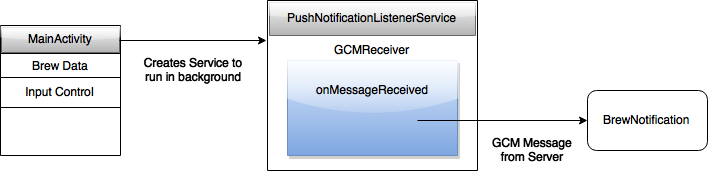
\includegraphics[scale=0.60]{gcm-push-notification.png}
\caption{Flow Design for Notification Service}
\label{fig:gcm-push-notification}
\end{center}
\end{figure}

\noindent MainActivity: This activity starts on application launch (when user taps on the app icon). The activity will start the PushNotificationListenerService to run in the background.

\noindent PushNotificationListenerService: The Listener uses the GCMReceiver class to listen for and to receive the data messages from the server. Whenever a \gls{json} message arrives to the client side, the onMessageReceived function is called to parse the \gls{json} message.

\noindent onMessageReceived: This function parses the \gls{json} message received by the Listener and creates a type of BrewNotification to display to the user.

\noindent BrewNotification: This object will encapsulate notification created for the end user. Types of BrewNotification are based on priority: max, medium and low. Max priority notification is given to messages that relay critical information about the brew system (overheat, pressure build up, etc). Medium priority notifications are created for important messages (brew changing state, brew completed). Low priority notifications are given to messages that contain messages which the user does not necessarily have to know (boil temperature reached).

\noindent To summarize, once the server sends a message to the client application,  the Listener service will process the message through the onMessageReceived function. Once the function parses which type of message it is, it displays the appropriate BrewNotification to the user.

\noindent The next part of the component displays previous data statistics recorded by the sensors on previous brews. The data displayed includes temperature readings, volume, sugar concentration and other sensor measurement. This gives the user the ability to look at past brews and possibly make adjustments. Figure \ref{fig:data-statistics} illustrates the application flow for the data statistics.

\begin{figure}[H]
\begin{center}
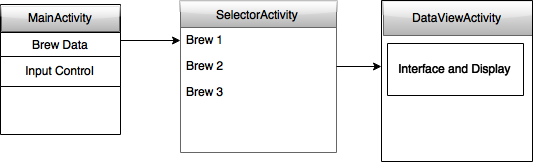
\includegraphics[scale=0.70]{data-statistics.png}
\caption{Flow Design for Data Statistics}
\label{fig:data-statistics}
\end{center}
\end{figure}

\noindent MainActivity: The main activity (same from the previous component) allows the user to launch the activity to select previous brews.

\noindent SelectorActivity: This activity contains a selectable list of all previously done brews. By selecting one item launches the DataViewActivity based on the brew.

\noindent DataViewActivity: Displays various data (temperature, pressure, yield percentage) of the brew selected by the user.
Providing this information allows the user to view and experiment with previous brews to enhance the quality of future brews. 

\noindent In conclusion, the real time data component of the application is designed to keep the user notified about the brew system, whether that would be about the current state of the brew process or about previous brew data. This enhances user experience such that the user does not have to constantly check the brew process to receive information since the system informs the user.

\subsubsection{Input Controls and Interaction}
The second component of the application is to allow the user to control the brew system with the mobile application. The goals of this component is to allow the user to start the brew process through the application and to provide control over various conditions within the brew process such as the maximum temperature, the target sugar concentration and others that would affect the brew's quality. Figure \ref{fig:input-activity} below shows the design flow for this component.

\begin{figure}[H]
\begin{center}
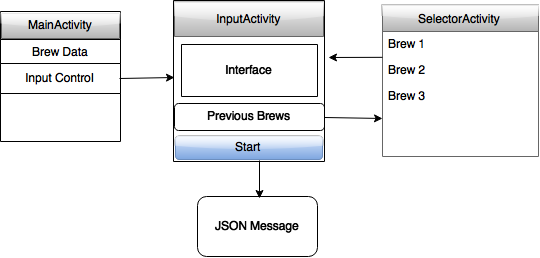
\includegraphics[scale=0.70]{input-activity.png}
\caption{Flow Design for User Input Activity}
\label{fig:input-activity}
\end{center}
\end{figure}

\noindent MainActivity: Option to select the input control activity, the main activity first checks if the mobile device is on the same local network as the vessel. If the device is not on the same network, the MainActivity will not allow the user to select the ``Input Controls" option. This is because the mobile application is designed to allow users to perform write applications only when connected on the same network as the web server, otherwise the application allows read-only operations. Although this will limit the application's usability, it ensures a high level of security on the brew system, where it does not allow others to exploit the application over the internet to cause the main vessel to malfunction. 

\noindent InputActivity: The InputActivity allows the user to select a previous brew process to modify or create a brand new brew process. The user can change various states such as max temperature for boils, number of hours and other conditions that might affect the brew. The user is also able to start the brew from the interface, by tapping the START button snapped to the bottom of the interface.

\noindent SelectorActivity: If the user selects a previous brew, the activity retrieves the relevant data from the server, and populate the interface of the InputActivity.

\noindent If the user taps the START button in the InputActivity interface, the application creates a \gls{json} file with all the data mapped to a key value. The client will send the \gls{json} file to the server and wait for a response. An error response from the server will have another key explaining the details of the error. The errors are based on lack of ingredients in the vessel or a malfunction detected by the system. A success response from the server means that the system started the brew.

\section{Discussion and Conclusions}
\subsection{Evaluation of Final Design}
The final design meets the objective and specifications listed in the project specification document. The combination of the subsystems creates an automated brew system that can control the climate within the vessel.  These controls are brought about by the inclusion of a temperature regulation which requires real-time temperature feedback to maintain precision. The functional requirements "Database" and "Application Notification" is implemented through a \gls{rest}Ful web server with various resources. There is also an additional specification to create a user interface so that the brewing device may be operated via a mobile device. 
\subsection{Use of Advanced Knowledge}
The subsystem designs all require upper year knowledge to complete. For developing the communications portion of the embedded computer system SELinux policies enforcing read only access is a crucial security precaution.  Proper security enforcement can minimize the potential for malicious attacks on the system as outlined in ECE 458, Computer Security.  Developing the Web Server and the Mobile Application includes knowledge from such courses as ECE356 (Database Systems), ECE454 (Distributed Systems) and ECE452 (Software Design and Architectures). Designing databases requires knowledge of various schemas, relations, normalization and indexing that are involved in the ECE356 contents. Designing a mobile application involves the knowledge of software design processes, methods and implementing those designs that is taught in ECE452. Finally, the brew system requires various sensor networks and communication between a centralized server to multiple clients which involves knowledge from ECE454. The design and analysis of the control systems used in the electrical subsystems require knowledge of control systems that are taught in both ECE380 and ECE 481, and the design and analysis of the power electronic components uses concepts take directly from ECE463.
\subsection{Creativity, Novelty, Elegance}
The novelty of our design is that it involves so many components from various Engineering backgrounds to complete. The system allows the user to have precise controls of the brew but at the same time offer flexibility in various environmental conditions during the process. One of the most elegant part of the project is that it takes the entire brew process and compacts it into one single vessel. The use of a double walled tank enables the heating and cooling apparatus to be mounted inside the device itself, adding to the singular design aspect of the fermenter.

\subsection{Quality of Risk Assessment}
\subsubsection{Assessed Risks}
The power electronic systems pose many hazards to the building of this system. The custom 120V circuitry is inherently dangerous to test, and proper precautions must be taken to avoid electrocution. The heating components of the system are capable of getting very hot, so proper care must be taken to avoid burns and potentially starting a fire. The motors can be very dangerous if anyone puts their hand near the spinning parts while the system is live, so it is important to make sure that everything is powered down and disconnected before attempting to adjust any of the motor actuated assemblies.

\pagebreak
\subsection{Student Workload}
Table below shows the amount of work contributed by each group member.
\begin{table}[H]
\centering
\caption{Project Contributions}
\label{workload-percentage}
\begin{tabular}{lr}
\toprule
\textbf{Group Member} 	& \textbf{Percentage of Workload}\\ 
\midrule
Kevin Nause (Embedded Systems)		&        25               \\
Mathieu Tremblay (Electrical)		&        25               \\
Scott Wood (Mechanical)				&        25               \\
Steve Jung (Mobile Application)		& 		 25				  \\
\bottomrule
\end{tabular}
\end{table}

The workload was divided on the various skills of each group member. Each group member was assigned a major component of the project based on their skills. 

\pagebreak

\printglossary[type=acronym]
\printglossary[type=beer]
\printglossary[type=technical]

\pagebreak

\bibliography{specifications-bib}{}
\bibliographystyle{ieeetr}

\pagebreak

\begin{appendices}
%Appendix A
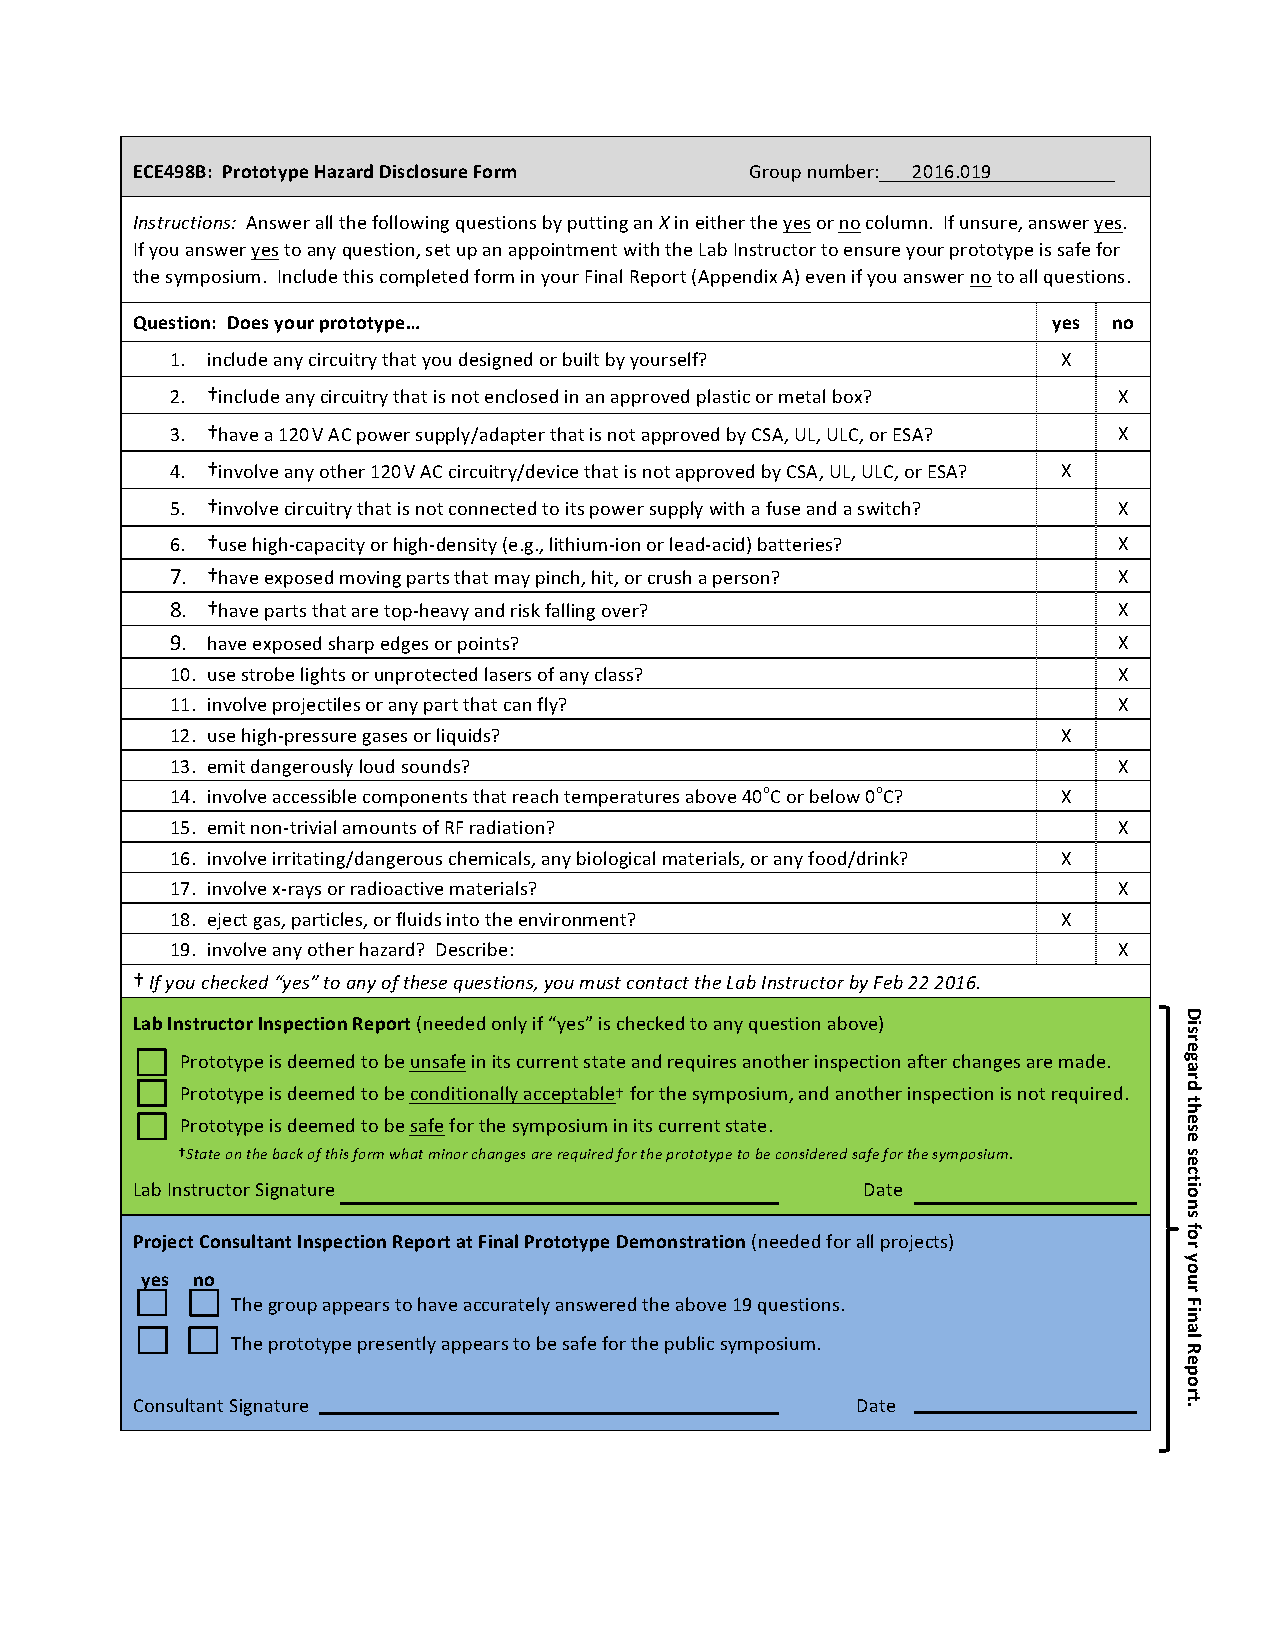
\includepdf[scale=0.9,pages=1,pagecommand=\section{Prototype Hazard Disclosure}]{forms/symposium_prototype_hazard_disclosure_form.pdf}

%Appendix B
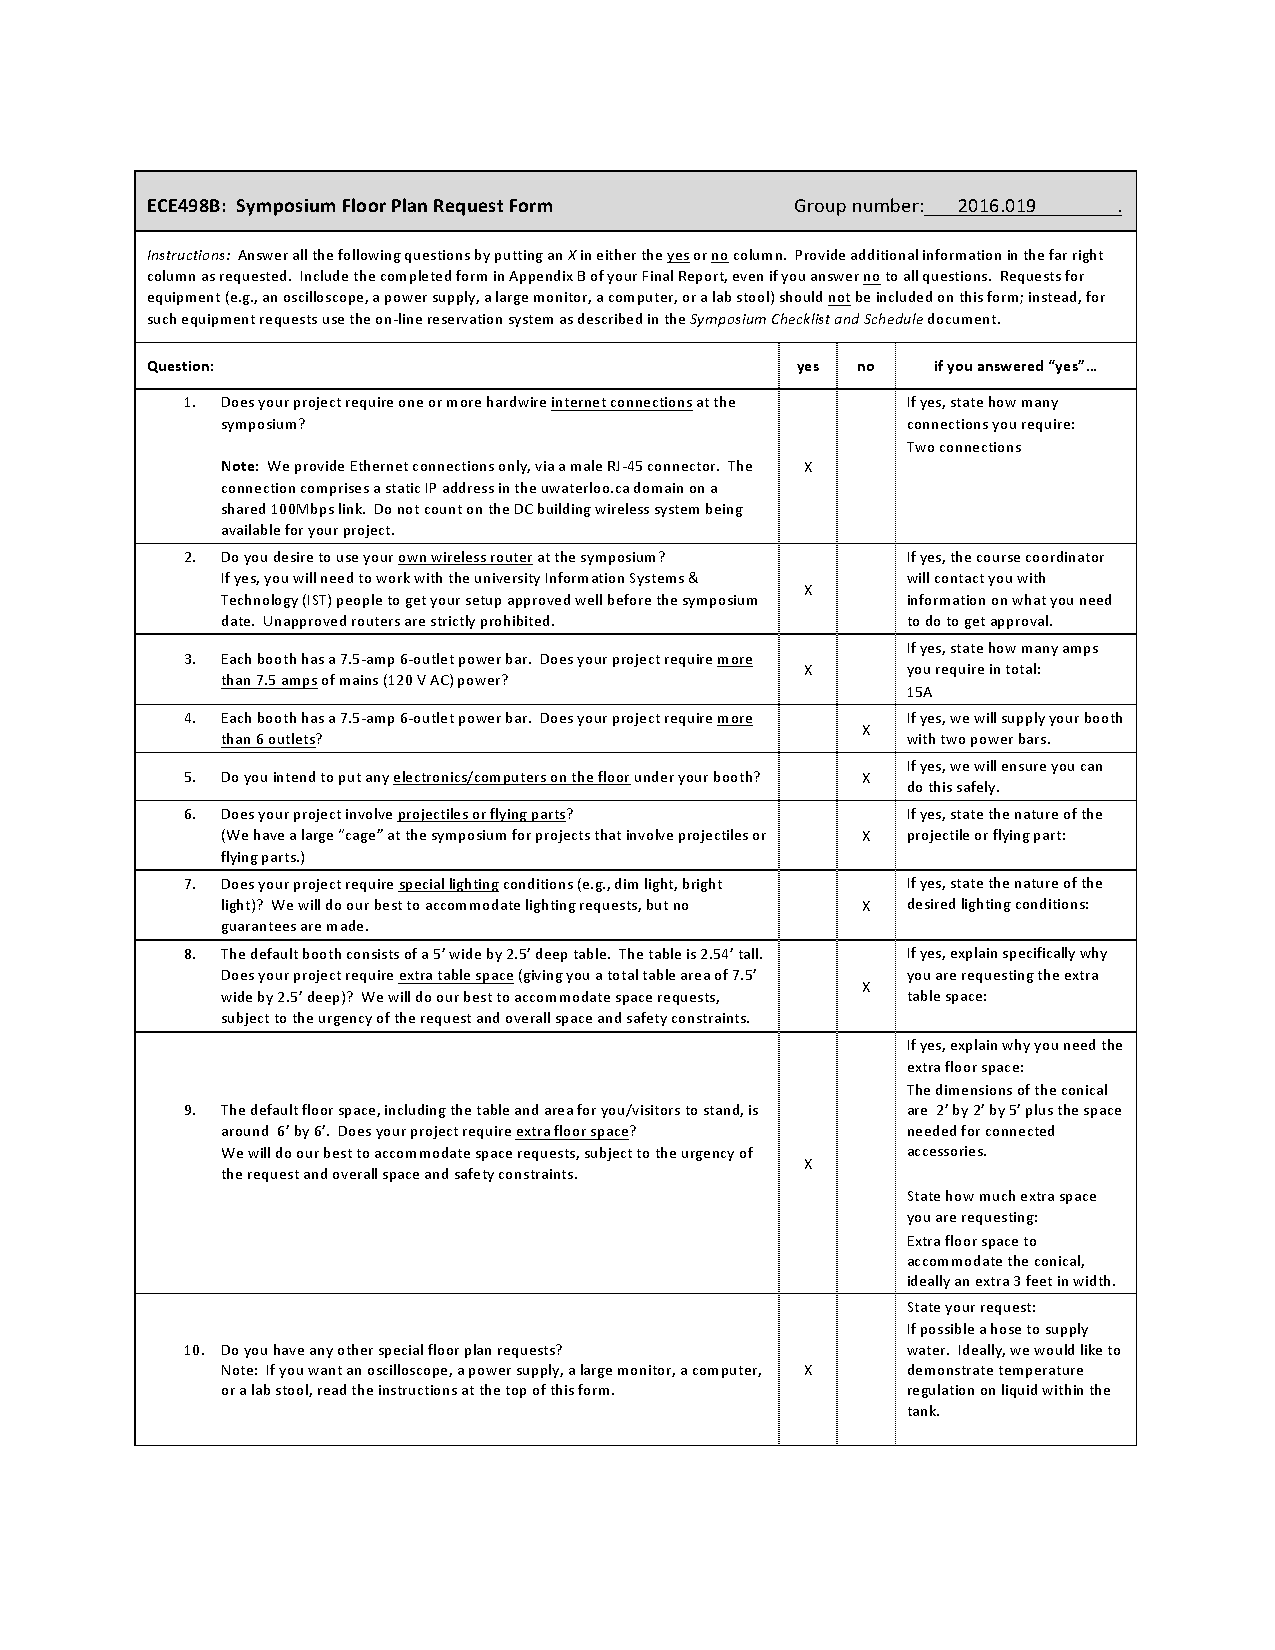
\includepdf[scale=0.9,pages=1,pagecommand=\section{Symposium Floor Plan Request}]{forms/symposium_floor_plan_request_form.pdf}

\section{Mechanical Materials}\label{app:304}
This section contains important lookup values for mechanical and materials calculations.
\begin{table}[H]
\caption{Alloying elements of \gls{aisi} 304 Stainless Steel \cite{machinery-handbook}}
\centering
\begin{tabularx}{\textwidth}{l l l l l l l l l Z}
\toprule
\textbf{Alloying Element} & Cr    & Ni     & C          & Mn        & Si         & P           & S           & N         \\
\textbf{Wt. \%}           & 18-20 & 8-10.5 & 0.08* & 2.0* & 0.75* & 0.045* & 0.030* & 0.10*\\
\bottomrule
\end{tabularx}
* Indicates maximum
\end{table}
\begin{table}[H]
\caption{\gls{aisi} Type 304 Stainless Steel Mechanical Properties \cite{matweb}}
\centering
\begin{tabularx}{\textwidth}{llllllZ}
\toprule
\textbf{\gls{yieldstr}} & \textbf{UTS}    & \textbf{Elasticity}        & \textbf{Poisson Ratio} & \textbf{Hardness} & \textbf{ Conductivity} & \textbf{Heat Capacity} \\ 
215 MPa      & \multicolumn{1}{l}{505 MPa} & \multicolumn{1}{l}{193 MPa} & 0.29            & 123               & 16.2 W/m-K           & 0.5 J/g$^{\circ}$C              \\
\bottomrule
\end{tabularx}
\end{table}

\begin{table}[H]
\caption{Alloying elements of 5052 Aluminium \cite{machinery-handbook}}
\centering
\begin{tabularx}{\textwidth}{lllllllZ}
\toprule
\textbf{Alloying Element} & Cr        & Cu        & Fe         & Mn        & Mg        & Zn        & Si         \\
\textbf{Wt. \%}           & 0.15-0.35 & 0.1* & 0.04* & 0.1* & 2.2 – 2.8 & 0.1* & 0.25* \\
\bottomrule
\end{tabularx}
* Indicates maximum
\end{table}

\begin{table}[H]
\caption{Type 5052 Aluminium Mechanical Properties \cite{matweb}}
\centering 
\begin{tabularx}{\textwidth}{llllllZ}
\toprule
\textbf{\gls{yieldstr}} & \textbf{UTS}    & \textbf{Elasticity}        & \textbf{Poisson Ratio} & \textbf{Hardness} & \textbf{ Conductivity} & \textbf{Heat Capacity} \\
193 MPa      & \multicolumn{1}{l}{228 MPa} & \multicolumn{1}{l}{70.3 MPa} & 0.33            & 60                & 138 W/m-K            & 0.88 J/g$^{\circ}$C \\
\bottomrule
\end{tabularx}
\label{tab:}
\end{table}

\end{appendices}
\end{document}
